
% Default to the notebook output style

    


% Inherit from the specified cell style.




    
\documentclass{report}

    
    
    \usepackage[T1]{fontenc}
    % Nicer default font (+ math font) than Computer Modern for most use cases
    \usepackage{mathpazo}

    % Basic figure setup, for now with no caption control since it's done
    % automatically by Pandoc (which extracts ![](path) syntax from Markdown).
    \usepackage{graphicx}
    % We will generate all images so they have a width \maxwidth. This means
    % that they will get their normal width if they fit onto the page, but
    % are scaled down if they would overflow the margins.
    \makeatletter
    \def\maxwidth{\ifdim\Gin@nat@width>\linewidth\linewidth
    \else\Gin@nat@width\fi}
    \makeatother
    \let\Oldincludegraphics\includegraphics
    % Set max figure width to be 80% of text width, for now hardcoded.
    \renewcommand{\includegraphics}[1]{\Oldincludegraphics[width=.8\maxwidth]{#1}}
    % Ensure that by default, figures have no caption (until we provide a
    % proper Figure object with a Caption API and a way to capture that
    % in the conversion process - todo).
    \usepackage{caption}
    \DeclareCaptionLabelFormat{nolabel}{}
    \captionsetup{labelformat=nolabel}

    \usepackage{adjustbox} % Used to constrain images to a maximum size 
    \usepackage{xcolor} % Allow colors to be defined
    \usepackage{enumerate} % Needed for markdown enumerations to work
    \usepackage{geometry} % Used to adjust the document margins
    \usepackage{amsmath} % Equations
    \usepackage{amssymb} % Equations
    \usepackage{textcomp} % defines textquotesingle
    % Hack from http://tex.stackexchange.com/a/47451/13684:
    \AtBeginDocument{%
        \def\PYZsq{\textquotesingle}% Upright quotes in Pygmentized code
    }
    \usepackage{upquote} % Upright quotes for verbatim code
    \usepackage{eurosym} % defines \euro
    \usepackage[mathletters]{ucs} % Extended unicode (utf-8) support
    \usepackage[utf8x]{inputenc} % Allow utf-8 characters in the tex document
    \usepackage{fancyvrb} % verbatim replacement that allows latex
    \usepackage{grffile} % extends the file name processing of package graphics 
                         % to support a larger range 
    % The hyperref package gives us a pdf with properly built
    % internal navigation ('pdf bookmarks' for the table of contents,
    % internal cross-reference links, web links for URLs, etc.)
    \usepackage{hyperref}
    \usepackage{longtable} % longtable support required by pandoc >1.10
    \usepackage{booktabs}  % table support for pandoc > 1.12.2
    \usepackage[inline]{enumitem} % IRkernel/repr support (it uses the enumerate* environment)
    \usepackage[normalem]{ulem} % ulem is needed to support strikethroughs (\sout)
                                % normalem makes italics be italics, not underlines
    

    
    
    % Colors for the hyperref package
    \definecolor{urlcolor}{rgb}{0,.145,.698}
    \definecolor{linkcolor}{rgb}{.71,0.21,0.01}
    \definecolor{citecolor}{rgb}{.12,.54,.11}

    % ANSI colors
    \definecolor{ansi-black}{HTML}{3E424D}
    \definecolor{ansi-black-intense}{HTML}{282C36}
    \definecolor{ansi-red}{HTML}{E75C58}
    \definecolor{ansi-red-intense}{HTML}{B22B31}
    \definecolor{ansi-green}{HTML}{00A250}
    \definecolor{ansi-green-intense}{HTML}{007427}
    \definecolor{ansi-yellow}{HTML}{DDB62B}
    \definecolor{ansi-yellow-intense}{HTML}{B27D12}
    \definecolor{ansi-blue}{HTML}{208FFB}
    \definecolor{ansi-blue-intense}{HTML}{0065CA}
    \definecolor{ansi-magenta}{HTML}{D160C4}
    \definecolor{ansi-magenta-intense}{HTML}{A03196}
    \definecolor{ansi-cyan}{HTML}{60C6C8}
    \definecolor{ansi-cyan-intense}{HTML}{258F8F}
    \definecolor{ansi-white}{HTML}{C5C1B4}
    \definecolor{ansi-white-intense}{HTML}{A1A6B2}

    % commands and environments needed by pandoc snippets
    % extracted from the output of `pandoc -s`
    \providecommand{\tightlist}{%
      \setlength{\itemsep}{0pt}\setlength{\parskip}{0pt}}
    \DefineVerbatimEnvironment{Highlighting}{Verbatim}{commandchars=\\\{\}}
    % Add ',fontsize=\small' for more characters per line
    \newenvironment{Shaded}{}{}
    \newcommand{\KeywordTok}[1]{\textcolor[rgb]{0.00,0.44,0.13}{\textbf{{#1}}}}
    \newcommand{\DataTypeTok}[1]{\textcolor[rgb]{0.56,0.13,0.00}{{#1}}}
    \newcommand{\DecValTok}[1]{\textcolor[rgb]{0.25,0.63,0.44}{{#1}}}
    \newcommand{\BaseNTok}[1]{\textcolor[rgb]{0.25,0.63,0.44}{{#1}}}
    \newcommand{\FloatTok}[1]{\textcolor[rgb]{0.25,0.63,0.44}{{#1}}}
    \newcommand{\CharTok}[1]{\textcolor[rgb]{0.25,0.44,0.63}{{#1}}}
    \newcommand{\StringTok}[1]{\textcolor[rgb]{0.25,0.44,0.63}{{#1}}}
    \newcommand{\CommentTok}[1]{\textcolor[rgb]{0.38,0.63,0.69}{\textit{{#1}}}}
    \newcommand{\OtherTok}[1]{\textcolor[rgb]{0.00,0.44,0.13}{{#1}}}
    \newcommand{\AlertTok}[1]{\textcolor[rgb]{1.00,0.00,0.00}{\textbf{{#1}}}}
    \newcommand{\FunctionTok}[1]{\textcolor[rgb]{0.02,0.16,0.49}{{#1}}}
    \newcommand{\RegionMarkerTok}[1]{{#1}}
    \newcommand{\ErrorTok}[1]{\textcolor[rgb]{1.00,0.00,0.00}{\textbf{{#1}}}}
    \newcommand{\NormalTok}[1]{{#1}}
    
    % Additional commands for more recent versions of Pandoc
    \newcommand{\ConstantTok}[1]{\textcolor[rgb]{0.53,0.00,0.00}{{#1}}}
    \newcommand{\SpecialCharTok}[1]{\textcolor[rgb]{0.25,0.44,0.63}{{#1}}}
    \newcommand{\VerbatimStringTok}[1]{\textcolor[rgb]{0.25,0.44,0.63}{{#1}}}
    \newcommand{\SpecialStringTok}[1]{\textcolor[rgb]{0.73,0.40,0.53}{{#1}}}
    \newcommand{\ImportTok}[1]{{#1}}
    \newcommand{\DocumentationTok}[1]{\textcolor[rgb]{0.73,0.13,0.13}{\textit{{#1}}}}
    \newcommand{\AnnotationTok}[1]{\textcolor[rgb]{0.38,0.63,0.69}{\textbf{\textit{{#1}}}}}
    \newcommand{\CommentVarTok}[1]{\textcolor[rgb]{0.38,0.63,0.69}{\textbf{\textit{{#1}}}}}
    \newcommand{\VariableTok}[1]{\textcolor[rgb]{0.10,0.09,0.49}{{#1}}}
    \newcommand{\ControlFlowTok}[1]{\textcolor[rgb]{0.00,0.44,0.13}{\textbf{{#1}}}}
    \newcommand{\OperatorTok}[1]{\textcolor[rgb]{0.40,0.40,0.40}{{#1}}}
    \newcommand{\BuiltInTok}[1]{{#1}}
    \newcommand{\ExtensionTok}[1]{{#1}}
    \newcommand{\PreprocessorTok}[1]{\textcolor[rgb]{0.74,0.48,0.00}{{#1}}}
    \newcommand{\AttributeTok}[1]{\textcolor[rgb]{0.49,0.56,0.16}{{#1}}}
    \newcommand{\InformationTok}[1]{\textcolor[rgb]{0.38,0.63,0.69}{\textbf{\textit{{#1}}}}}
    \newcommand{\WarningTok}[1]{\textcolor[rgb]{0.38,0.63,0.69}{\textbf{\textit{{#1}}}}}
    
    
    % Define a nice break command that doesn't care if a line doesn't already
    % exist.
    \def\br{\hspace*{\fill} \\* }
    % Math Jax compatability definitions
    \def\gt{>}
    \def\lt{<}
    % Document parameters
    \title{Neuromorphic\_Silicon\_Photonics}
    
    
    

    % Pygments definitions
    
\makeatletter
\def\PY@reset{\let\PY@it=\relax \let\PY@bf=\relax%
    \let\PY@ul=\relax \let\PY@tc=\relax%
    \let\PY@bc=\relax \let\PY@ff=\relax}
\def\PY@tok#1{\csname PY@tok@#1\endcsname}
\def\PY@toks#1+{\ifx\relax#1\empty\else%
    \PY@tok{#1}\expandafter\PY@toks\fi}
\def\PY@do#1{\PY@bc{\PY@tc{\PY@ul{%
    \PY@it{\PY@bf{\PY@ff{#1}}}}}}}
\def\PY#1#2{\PY@reset\PY@toks#1+\relax+\PY@do{#2}}

\expandafter\def\csname PY@tok@w\endcsname{\def\PY@tc##1{\textcolor[rgb]{0.73,0.73,0.73}{##1}}}
\expandafter\def\csname PY@tok@c\endcsname{\let\PY@it=\textit\def\PY@tc##1{\textcolor[rgb]{0.25,0.50,0.50}{##1}}}
\expandafter\def\csname PY@tok@cp\endcsname{\def\PY@tc##1{\textcolor[rgb]{0.74,0.48,0.00}{##1}}}
\expandafter\def\csname PY@tok@k\endcsname{\let\PY@bf=\textbf\def\PY@tc##1{\textcolor[rgb]{0.00,0.50,0.00}{##1}}}
\expandafter\def\csname PY@tok@kp\endcsname{\def\PY@tc##1{\textcolor[rgb]{0.00,0.50,0.00}{##1}}}
\expandafter\def\csname PY@tok@kt\endcsname{\def\PY@tc##1{\textcolor[rgb]{0.69,0.00,0.25}{##1}}}
\expandafter\def\csname PY@tok@o\endcsname{\def\PY@tc##1{\textcolor[rgb]{0.40,0.40,0.40}{##1}}}
\expandafter\def\csname PY@tok@ow\endcsname{\let\PY@bf=\textbf\def\PY@tc##1{\textcolor[rgb]{0.67,0.13,1.00}{##1}}}
\expandafter\def\csname PY@tok@nb\endcsname{\def\PY@tc##1{\textcolor[rgb]{0.00,0.50,0.00}{##1}}}
\expandafter\def\csname PY@tok@nf\endcsname{\def\PY@tc##1{\textcolor[rgb]{0.00,0.00,1.00}{##1}}}
\expandafter\def\csname PY@tok@nc\endcsname{\let\PY@bf=\textbf\def\PY@tc##1{\textcolor[rgb]{0.00,0.00,1.00}{##1}}}
\expandafter\def\csname PY@tok@nn\endcsname{\let\PY@bf=\textbf\def\PY@tc##1{\textcolor[rgb]{0.00,0.00,1.00}{##1}}}
\expandafter\def\csname PY@tok@ne\endcsname{\let\PY@bf=\textbf\def\PY@tc##1{\textcolor[rgb]{0.82,0.25,0.23}{##1}}}
\expandafter\def\csname PY@tok@nv\endcsname{\def\PY@tc##1{\textcolor[rgb]{0.10,0.09,0.49}{##1}}}
\expandafter\def\csname PY@tok@no\endcsname{\def\PY@tc##1{\textcolor[rgb]{0.53,0.00,0.00}{##1}}}
\expandafter\def\csname PY@tok@nl\endcsname{\def\PY@tc##1{\textcolor[rgb]{0.63,0.63,0.00}{##1}}}
\expandafter\def\csname PY@tok@ni\endcsname{\let\PY@bf=\textbf\def\PY@tc##1{\textcolor[rgb]{0.60,0.60,0.60}{##1}}}
\expandafter\def\csname PY@tok@na\endcsname{\def\PY@tc##1{\textcolor[rgb]{0.49,0.56,0.16}{##1}}}
\expandafter\def\csname PY@tok@nt\endcsname{\let\PY@bf=\textbf\def\PY@tc##1{\textcolor[rgb]{0.00,0.50,0.00}{##1}}}
\expandafter\def\csname PY@tok@nd\endcsname{\def\PY@tc##1{\textcolor[rgb]{0.67,0.13,1.00}{##1}}}
\expandafter\def\csname PY@tok@s\endcsname{\def\PY@tc##1{\textcolor[rgb]{0.73,0.13,0.13}{##1}}}
\expandafter\def\csname PY@tok@sd\endcsname{\let\PY@it=\textit\def\PY@tc##1{\textcolor[rgb]{0.73,0.13,0.13}{##1}}}
\expandafter\def\csname PY@tok@si\endcsname{\let\PY@bf=\textbf\def\PY@tc##1{\textcolor[rgb]{0.73,0.40,0.53}{##1}}}
\expandafter\def\csname PY@tok@se\endcsname{\let\PY@bf=\textbf\def\PY@tc##1{\textcolor[rgb]{0.73,0.40,0.13}{##1}}}
\expandafter\def\csname PY@tok@sr\endcsname{\def\PY@tc##1{\textcolor[rgb]{0.73,0.40,0.53}{##1}}}
\expandafter\def\csname PY@tok@ss\endcsname{\def\PY@tc##1{\textcolor[rgb]{0.10,0.09,0.49}{##1}}}
\expandafter\def\csname PY@tok@sx\endcsname{\def\PY@tc##1{\textcolor[rgb]{0.00,0.50,0.00}{##1}}}
\expandafter\def\csname PY@tok@m\endcsname{\def\PY@tc##1{\textcolor[rgb]{0.40,0.40,0.40}{##1}}}
\expandafter\def\csname PY@tok@gh\endcsname{\let\PY@bf=\textbf\def\PY@tc##1{\textcolor[rgb]{0.00,0.00,0.50}{##1}}}
\expandafter\def\csname PY@tok@gu\endcsname{\let\PY@bf=\textbf\def\PY@tc##1{\textcolor[rgb]{0.50,0.00,0.50}{##1}}}
\expandafter\def\csname PY@tok@gd\endcsname{\def\PY@tc##1{\textcolor[rgb]{0.63,0.00,0.00}{##1}}}
\expandafter\def\csname PY@tok@gi\endcsname{\def\PY@tc##1{\textcolor[rgb]{0.00,0.63,0.00}{##1}}}
\expandafter\def\csname PY@tok@gr\endcsname{\def\PY@tc##1{\textcolor[rgb]{1.00,0.00,0.00}{##1}}}
\expandafter\def\csname PY@tok@ge\endcsname{\let\PY@it=\textit}
\expandafter\def\csname PY@tok@gs\endcsname{\let\PY@bf=\textbf}
\expandafter\def\csname PY@tok@gp\endcsname{\let\PY@bf=\textbf\def\PY@tc##1{\textcolor[rgb]{0.00,0.00,0.50}{##1}}}
\expandafter\def\csname PY@tok@go\endcsname{\def\PY@tc##1{\textcolor[rgb]{0.53,0.53,0.53}{##1}}}
\expandafter\def\csname PY@tok@gt\endcsname{\def\PY@tc##1{\textcolor[rgb]{0.00,0.27,0.87}{##1}}}
\expandafter\def\csname PY@tok@err\endcsname{\def\PY@bc##1{\setlength{\fboxsep}{0pt}\fcolorbox[rgb]{1.00,0.00,0.00}{1,1,1}{\strut ##1}}}
\expandafter\def\csname PY@tok@kc\endcsname{\let\PY@bf=\textbf\def\PY@tc##1{\textcolor[rgb]{0.00,0.50,0.00}{##1}}}
\expandafter\def\csname PY@tok@kd\endcsname{\let\PY@bf=\textbf\def\PY@tc##1{\textcolor[rgb]{0.00,0.50,0.00}{##1}}}
\expandafter\def\csname PY@tok@kn\endcsname{\let\PY@bf=\textbf\def\PY@tc##1{\textcolor[rgb]{0.00,0.50,0.00}{##1}}}
\expandafter\def\csname PY@tok@kr\endcsname{\let\PY@bf=\textbf\def\PY@tc##1{\textcolor[rgb]{0.00,0.50,0.00}{##1}}}
\expandafter\def\csname PY@tok@bp\endcsname{\def\PY@tc##1{\textcolor[rgb]{0.00,0.50,0.00}{##1}}}
\expandafter\def\csname PY@tok@fm\endcsname{\def\PY@tc##1{\textcolor[rgb]{0.00,0.00,1.00}{##1}}}
\expandafter\def\csname PY@tok@vc\endcsname{\def\PY@tc##1{\textcolor[rgb]{0.10,0.09,0.49}{##1}}}
\expandafter\def\csname PY@tok@vg\endcsname{\def\PY@tc##1{\textcolor[rgb]{0.10,0.09,0.49}{##1}}}
\expandafter\def\csname PY@tok@vi\endcsname{\def\PY@tc##1{\textcolor[rgb]{0.10,0.09,0.49}{##1}}}
\expandafter\def\csname PY@tok@vm\endcsname{\def\PY@tc##1{\textcolor[rgb]{0.10,0.09,0.49}{##1}}}
\expandafter\def\csname PY@tok@sa\endcsname{\def\PY@tc##1{\textcolor[rgb]{0.73,0.13,0.13}{##1}}}
\expandafter\def\csname PY@tok@sb\endcsname{\def\PY@tc##1{\textcolor[rgb]{0.73,0.13,0.13}{##1}}}
\expandafter\def\csname PY@tok@sc\endcsname{\def\PY@tc##1{\textcolor[rgb]{0.73,0.13,0.13}{##1}}}
\expandafter\def\csname PY@tok@dl\endcsname{\def\PY@tc##1{\textcolor[rgb]{0.73,0.13,0.13}{##1}}}
\expandafter\def\csname PY@tok@s2\endcsname{\def\PY@tc##1{\textcolor[rgb]{0.73,0.13,0.13}{##1}}}
\expandafter\def\csname PY@tok@sh\endcsname{\def\PY@tc##1{\textcolor[rgb]{0.73,0.13,0.13}{##1}}}
\expandafter\def\csname PY@tok@s1\endcsname{\def\PY@tc##1{\textcolor[rgb]{0.73,0.13,0.13}{##1}}}
\expandafter\def\csname PY@tok@mb\endcsname{\def\PY@tc##1{\textcolor[rgb]{0.40,0.40,0.40}{##1}}}
\expandafter\def\csname PY@tok@mf\endcsname{\def\PY@tc##1{\textcolor[rgb]{0.40,0.40,0.40}{##1}}}
\expandafter\def\csname PY@tok@mh\endcsname{\def\PY@tc##1{\textcolor[rgb]{0.40,0.40,0.40}{##1}}}
\expandafter\def\csname PY@tok@mi\endcsname{\def\PY@tc##1{\textcolor[rgb]{0.40,0.40,0.40}{##1}}}
\expandafter\def\csname PY@tok@il\endcsname{\def\PY@tc##1{\textcolor[rgb]{0.40,0.40,0.40}{##1}}}
\expandafter\def\csname PY@tok@mo\endcsname{\def\PY@tc##1{\textcolor[rgb]{0.40,0.40,0.40}{##1}}}
\expandafter\def\csname PY@tok@ch\endcsname{\let\PY@it=\textit\def\PY@tc##1{\textcolor[rgb]{0.25,0.50,0.50}{##1}}}
\expandafter\def\csname PY@tok@cm\endcsname{\let\PY@it=\textit\def\PY@tc##1{\textcolor[rgb]{0.25,0.50,0.50}{##1}}}
\expandafter\def\csname PY@tok@cpf\endcsname{\let\PY@it=\textit\def\PY@tc##1{\textcolor[rgb]{0.25,0.50,0.50}{##1}}}
\expandafter\def\csname PY@tok@c1\endcsname{\let\PY@it=\textit\def\PY@tc##1{\textcolor[rgb]{0.25,0.50,0.50}{##1}}}
\expandafter\def\csname PY@tok@cs\endcsname{\let\PY@it=\textit\def\PY@tc##1{\textcolor[rgb]{0.25,0.50,0.50}{##1}}}

\def\PYZbs{\char`\\}
\def\PYZus{\char`\_}
\def\PYZob{\char`\{}
\def\PYZcb{\char`\}}
\def\PYZca{\char`\^}
\def\PYZam{\char`\&}
\def\PYZlt{\char`\<}
\def\PYZgt{\char`\>}
\def\PYZsh{\char`\#}
\def\PYZpc{\char`\%}
\def\PYZdl{\char`\$}
\def\PYZhy{\char`\-}
\def\PYZsq{\char`\'}
\def\PYZdq{\char`\"}
\def\PYZti{\char`\~}
% for compatibility with earlier versions
\def\PYZat{@}
\def\PYZlb{[}
\def\PYZrb{]}
\makeatother


    % Exact colors from NB
    \definecolor{incolor}{rgb}{0.0, 0.0, 0.5}
    \definecolor{outcolor}{rgb}{0.545, 0.0, 0.0}



    
    % Prevent overflowing lines due to hard-to-break entities
    \sloppy 
    % Setup hyperref package
    \hypersetup{
      breaklinks=true,  % so long urls are correctly broken across lines
      colorlinks=true,
      urlcolor=urlcolor,
      linkcolor=linkcolor,
      citecolor=citecolor,
      }
    % Slightly bigger margins than the latex defaults
    
    \geometry{verbose,tmargin=1in,bmargin=1in,lmargin=1in,rmargin=1in}
    
    

    \begin{document}
    
    
    
    \maketitle
    
    
    \tableofcontents


    
\chapter{Solving ODEs with Photonic Modulator
Neurons}\label{solving-odes-with-photonic-modulator-neurons}

This notebook was created to support the publication of an article
titled \href{https://arxiv.org/abs/1611.02272}{\emph{Neuromorphic
Silicon Photonics}}, authored by Alexander N. Tait, Ellen Zhou, Thomas
Ferreira de Lima, Allie X. Wu, Mitchell A. Nahmias, Bhavin J. Shastri
and Paul R. Prucnal, first submitted on 5 Nov 2016.

A copy of this notebook is available at:

https://github.com/lightwave-lab/Neuromorphic\_Silicon\_Photonics

    \begin{Verbatim}[commandchars=\\\{\}]
{\color{incolor}In [{\color{incolor}1}]:} \PY{c+c1}{\PYZsh{} The following notebook was run using Python 3.6.0 and nengo 2.2.0}
        \PY{c+c1}{\PYZsh{} Setting up notebook}
        \PY{k+kn}{import} \PY{n+nn}{numpy} \PY{k}{as} \PY{n+nn}{np}
        \PY{k+kn}{import} \PY{n+nn}{matplotlib}\PY{n+nn}{.}\PY{n+nn}{pyplot} \PY{k}{as} \PY{n+nn}{plt}
        \PY{k+kn}{import} \PY{n+nn}{matplotlib}\PY{n+nn}{.}\PY{n+nn}{colors} \PY{k}{as} \PY{n+nn}{colors}
        \PY{k+kn}{import} \PY{n+nn}{matplotlib}\PY{n+nn}{.}\PY{n+nn}{cm} \PY{k}{as} \PY{n+nn}{cmx}
        \PY{o}{\PYZpc{}}\PY{k}{matplotlib} inline
        \PY{k+kn}{from} \PY{n+nn}{matplotlib}\PY{n+nn}{.}\PY{n+nn}{backends}\PY{n+nn}{.}\PY{n+nn}{backend\PYZus{}pdf} \PY{k}{import} \PY{n}{PdfPages}
        \PY{o}{\PYZpc{}}\PY{k}{config} InlineBackend.figure\PYZus{}format = \PYZsq{}retina\PYZsq{}
        
        \PY{n}{plt}\PY{o}{.}\PY{n}{style}\PY{o}{.}\PY{n}{use}\PY{p}{(}\PY{l+s+s1}{\PYZsq{}}\PY{l+s+s1}{seaborn\PYZhy{}colorblind}\PY{l+s+s1}{\PYZsq{}}\PY{p}{)}
        
        \PY{k+kn}{from} \PY{n+nn}{matplotlib} \PY{k}{import} \PY{n}{rc}\PY{p}{,} \PY{n}{rcParams}
        \PY{n}{rc}\PY{p}{(}\PY{l+s+s1}{\PYZsq{}}\PY{l+s+s1}{font}\PY{l+s+s1}{\PYZsq{}}\PY{p}{,}\PY{o}{*}\PY{o}{*}\PY{p}{\PYZob{}}\PY{l+s+s1}{\PYZsq{}}\PY{l+s+s1}{family}\PY{l+s+s1}{\PYZsq{}}\PY{p}{:}\PY{l+s+s1}{\PYZsq{}}\PY{l+s+s1}{sans\PYZhy{}serif}\PY{l+s+s1}{\PYZsq{}}\PY{p}{,}\PY{l+s+s1}{\PYZsq{}}\PY{l+s+s1}{sans\PYZhy{}serif}\PY{l+s+s1}{\PYZsq{}}\PY{p}{:}\PY{p}{[}\PY{l+s+s1}{\PYZsq{}}\PY{l+s+s1}{Helvetica}\PY{l+s+s1}{\PYZsq{}}\PY{p}{]}\PY{p}{,}\PY{l+s+s1}{\PYZsq{}}\PY{l+s+s1}{size}\PY{l+s+s1}{\PYZsq{}}\PY{p}{:}\PY{l+m+mi}{7}\PY{p}{\PYZcb{}}\PY{p}{)}
        \PY{n}{rc}\PY{p}{(}\PY{l+s+s1}{\PYZsq{}}\PY{l+s+s1}{text}\PY{l+s+s1}{\PYZsq{}}\PY{p}{,} \PY{n}{usetex}\PY{o}{=}\PY{k+kc}{True}\PY{p}{)}
        \PY{n}{rcParams}\PY{p}{[}\PY{l+s+s1}{\PYZsq{}}\PY{l+s+s1}{text.latex.preamble}\PY{l+s+s1}{\PYZsq{}}\PY{p}{]} \PY{o}{=} \PY{p}{[}\PY{l+s+sa}{r}\PY{l+s+s1}{\PYZsq{}}\PY{l+s+s1}{\PYZbs{}}\PY{l+s+s1}{usepackage}\PY{l+s+si}{\PYZob{}sfmath\PYZcb{}}\PY{l+s+s1}{\PYZsq{}}\PY{p}{]}
        
        \PY{k+kn}{import} \PY{n+nn}{nengo}
        \PY{o}{\PYZpc{}}\PY{k}{load\PYZus{}ext} nengo.ipynb
\end{Verbatim}

    
    \begin{verbatim}
<IPython.core.display.Javascript object>
    \end{verbatim}

    
\section{Modifications to the nengo
project}\label{modifications-to-the-nengo-project}

Nengo is based exclusively on monotonic, non-negative output neuron
models. However, its encoding-decoding algorithms should work with other
kinds of neuron models. Here, we use the following
\texttt{FourierSinusoid} class of neurons included in our fork of the
\href{https://github.com/nengo/nengo/}{nengo project}.

\begin{Shaded}
\begin{Highlighting}[]
\CommentTok{# In nengo/neurons.py}
\KeywordTok{class}\NormalTok{ FourierSinusoid(NeuronType):}
    \CommentTok{"""A neuron model whose response curve is a half-period of a}
\CommentTok{    sinusoidal curve.}

\CommentTok{    DISCLAIMER: This class was hijacked. The new interpretation of}
\CommentTok{    intercepts and max_rates are as follows is as follows:}
\CommentTok{    intercepts : phase at dot(x, e) = 0}
\CommentTok{        (-0.5, 0.5)}
\CommentTok{    max_rates : directly proportional to gain.}
\CommentTok{        i.e. how many periods do we want between dot(x, e) = -1 and 1}
\CommentTok{    """}

\NormalTok{    probeable }\OperatorTok{=}\NormalTok{ (}\StringTok{'rates'}\NormalTok{, )}

\NormalTok{    s_pi }\OperatorTok{=}\NormalTok{ NumberParam(}\StringTok{'s_pi'}\NormalTok{, low}\OperatorTok{=}\DecValTok{0}\NormalTok{)}

    \KeywordTok{def} \FunctionTok{__init__}\NormalTok{(}\VariableTok{self}\NormalTok{, max_overall_rate}\OperatorTok{=}\DecValTok{400}\NormalTok{, s_pi}\OperatorTok{=}\FloatTok{0.1}\NormalTok{):}
        \BuiltInTok{super}\NormalTok{(FourierSinusoid, }\VariableTok{self}\NormalTok{).}\FunctionTok{__init__}\NormalTok{()}
        \VariableTok{self}\NormalTok{.max_overall_rate }\OperatorTok{=}\NormalTok{ max_overall_rate}
        \VariableTok{self}\NormalTok{.s_pi }\OperatorTok{=}\NormalTok{ s_pi}

    \KeywordTok{def}\NormalTok{ gain_bias_old(}\VariableTok{self}\NormalTok{, max_rates, intercepts):}
        \CommentTok{"""Determine gain and bias by shifting and scaling the lines."""}

\NormalTok{        gain }\OperatorTok{=}\NormalTok{ max_rates }\OperatorTok{*} \VariableTok{self}\NormalTok{.s_pi}
        \ControlFlowTok{with}\NormalTok{ np.errstate(divide}\OperatorTok{=}\StringTok{'ignore'}\NormalTok{, invalid}\OperatorTok{=}\StringTok{'ignore'}\NormalTok{):}
\NormalTok{            bias }\OperatorTok{=}\NormalTok{ np.divide(intercepts, gain)}
\NormalTok{        bias }\OperatorTok{=}\NormalTok{ np.where(}\OperatorTok{~}\NormalTok{np.isfinite(np.}\BuiltInTok{abs}\NormalTok{(bias)), }\DecValTok{0}\NormalTok{, bias)}
        \ControlFlowTok{return}\NormalTok{ gain, bias}

    \KeywordTok{def}\NormalTok{ gain_bias(}\VariableTok{self}\NormalTok{, max_rates, intercepts):}
        \CommentTok{"""Determine gain and bias by shifting and scaling the lines.}
\CommentTok{        This one foregoes any calculation"""}
\NormalTok{        gain }\OperatorTok{=}\NormalTok{ max_rates}
\NormalTok{        bias }\OperatorTok{=}\NormalTok{ intercepts}
        \ControlFlowTok{return}\NormalTok{ gain, bias}

    \CommentTok{# def step_math_old(self, dt, J, output, voltage):}
    \CommentTok{#     """Implement the nonlinearity."""}
    \CommentTok{#     # basically the formula is output = 0.5*(1 + sin(J/s_pi * pi))}
    \CommentTok{#     voltage = J / self.s_pi}

    \CommentTok{#     output[...] = self.max_overall_rate * 0.5 * \textbackslash{}}
    \CommentTok{#         (1 + np.sin(np.pi * voltage))}

    \KeywordTok{def}\NormalTok{ step_math(}\VariableTok{self}\NormalTok{, dt, J, output):}
        \CommentTok{"""Implement the nonlinearity.}
\CommentTok{        This one allows for negative outputs"""}
        \CommentTok{# basically the formula is output = 0.5*(1 + sin(J/s_pi * pi))}
\NormalTok{        voltage }\OperatorTok{=}\NormalTok{ J }\OperatorTok{/} \VariableTok{self}\NormalTok{.s_pi}

\NormalTok{        output[...] }\OperatorTok{=} \VariableTok{self}\NormalTok{.max_overall_rate }\OperatorTok{*} \FloatTok{0.5} \OperatorTok{*}\NormalTok{ (np.sin(np.pi }\OperatorTok{*}\NormalTok{ voltage) }\OperatorTok{+} \DecValTok{1}\NormalTok{)}
\end{Highlighting}
\end{Shaded}

\section{The Lorenz chaotic
attractor}\label{the-lorenz-chaotic-attractor}

In this simulation, we chose to construct a neural network using the
neurons defined \protect\hyperlink{fourier_neuron_nengo}{above} to solve
a classical chaotic dynamical system named ``Lorenz attractor''.

The equations are:

\[
\dot{x}_0 = \nu(x_1 - x_0) \\
\dot{x}_1 = x_0 (\rho - x_2) - x_1  \\
\dot{x}_2 = x_0 x_1 - \beta x_2 
\]

Since \(x_2\) is centered around approximately \(\rho\), and since NEF
ensembles are usually optimized to represent values within a certain
radius of the origin, we substitute \(x_2' = x_2 - \rho\), giving these
equations: \[
\dot{x}_0 = \nu(x_1 - x_0) \\
\dot{x}_1 = - x_0 x_2' - x_1\\
\dot{x}_2' = x_0 x_1 - \beta (x_2' + \rho)
\]

Refer to the standard example of the Lorenz attractor solver with 2000
neurons in a
\href{https://github.com/nengo/nengo/blob/master/examples/dynamics/lorenz_attractor.ipynb}{nengo
example}. *Note that the last equation for \(x_2'\) is typically shown
with an error in that example and in other articles from
Prof.~Eliasmith's group.

\section{Encoding strategy}\label{encoding-strategy}

From here onwards, we will refer the Lorenz system in its reduced form
as as \(\vec x = f(\vec x)\), with:

\[
\vec x = [x_0, x_1, x_2']^T
\]

and

\[
f(\vec x) = \left[
\begin{array}{c}
\nu(x_1 - x_0) \\
- x_0 x_2'- x_1 \\
x_0 x_1 - \beta (x_2' + \rho)
\end{array}
\right]
\]

\subsection{Neuron model}\label{neuron-model}

Using \href{http://www.nengo.ca}{nengo}, we instantiate a population of
\(N\) neurons that are all-to-all interconnected. These neurons are
responsible of \emph{representing} the vector \(\vec x\) at any time
\(t\). We consider the state of each neuron as \(\vec s = [s_i]\) for
neuron \(i\). The ODE that models each neuron, in this case, is:

\[\tau s_i + s_i = u_i \] where \(u_i\) represents the post-synaptic
input of the neuron and \(y_i=\sigma(s_i)\) its output.

\subsection{Nengo encoding strategy}\label{nengo-encoding-strategy}

In order to \emph{encode} a vector \(\vec x\) in the population \(N\),
nengo performs the following linear transformation (it has to be linear
for the method to work):

\[ s_i = g_i \vec e_i \cdot \vec x + b_i \] where \(g_i\) is a gain
term, \(\vec e_i\) is an encoder vector, and \(b_i\) is a bias term.
This is called the \emph{encoding strategy}.

Nonlinear operations are effectively performed by linear combinations of
the neural nonlinearities \(\sigma(s_i)\). Therefore, it is the
encoder's mission to generate as much entropy about the variables
\(\vec x\) as possible. This can be done by generating a diverse set of
\((g, \vec e, b)\) parameters. Below, we do this by using
\(\vec e_i = [1, \pm 1, \pm1]\), mixing all components of \(\vec x\)
together. Note: this can be optimized even further by noticing that the
ODE does not contain \(x_0 x_2\) terms.

Because we know that \(\sigma\) is a sinusoid, we create a set of
\((g,b)\) values to span a Fourier-like basis of functions across the
domain \(\vec e_i \cdot \vec x \in [-1,1]\). (See
\protect\hyperlink{tuning_curves}{tuning curves}).

    \begin{Verbatim}[commandchars=\\\{\}]
{\color{incolor}In [{\color{incolor}2}]:} \PY{n}{model} \PY{o}{=} \PY{n}{nengo}\PY{o}{.}\PY{n}{Network}\PY{p}{(}\PY{p}{)}
        \PY{c+c1}{\PYZsh{} V\PYZus{}pi of a modulator converted to state variable}
        \PY{n}{s\PYZus{}pi} \PY{o}{=} \PY{l+m+mf}{0.1}
        \PY{c+c1}{\PYZsh{} Max rate, or output, which is transmission in this case}
        \PY{n}{max\PYZus{}transmission} \PY{o}{=} \PY{l+m+mi}{1}
        \PY{c+c1}{\PYZsh{} Intercept, in this case, corresponds to where the tuning curve intercepts}
        \PY{c+c1}{\PYZsh{} zero. Range of [\PYZhy{}.5, .5] corresponds to [\PYZhy{}pi, pi]}
        \PY{n}{ints} \PY{o}{=} \PY{p}{[}\PY{l+m+mi}{0}\PY{p}{,} \PY{l+m+mi}{1}\PY{o}{/}\PY{l+m+mi}{4}\PY{p}{]}
        \PY{c+c1}{\PYZsh{} This number represents how many periods do we want between \PYZhy{}1 and 1 }
        \PY{c+c1}{\PYZsh{} (see tuning curves below)}
        \PY{n}{rats} \PY{o}{=} \PY{n}{s\PYZus{}pi} \PY{o}{*} \PY{n}{np}\PY{o}{.}\PY{n}{arange}\PY{p}{(}\PY{l+m+mi}{1}\PY{p}{,} \PY{l+m+mi}{4}\PY{p}{)}\PY{o}{/}\PY{l+m+mi}{2}
        \PY{c+c1}{\PYZsh{} Encoder multipliers}
        \PY{n}{enst} \PY{o}{=} \PY{p}{[}\PY{o}{\PYZhy{}}\PY{l+m+mi}{1}\PY{p}{,}\PY{l+m+mi}{1}\PY{p}{]}
        
        \PY{n}{num\PYZus{}intercepts} \PY{o}{=} \PY{n+nb}{len}\PY{p}{(}\PY{n}{ints}\PY{p}{)}
        \PY{n}{num\PYZus{}max\PYZus{}rates} \PY{o}{=} \PY{n+nb}{len}\PY{p}{(}\PY{n}{rats}\PY{p}{)}
        \PY{n}{num\PYZus{}encoders} \PY{o}{=} \PY{n+nb}{len}\PY{p}{(}\PY{n}{enst}\PY{p}{)} \PY{o}{*}\PY{o}{*} \PY{l+m+mi}{2}
        
        \PY{c+c1}{\PYZsh{} Constant neuron}
        \PY{n}{constant\PYZus{}neuron} \PY{o}{=} \PY{k+kc}{False}
        \PY{n}{num\PYZus{}neurons} \PY{o}{=} \PY{n}{np}\PY{o}{.}\PY{n}{int\PYZus{}}\PY{p}{(}\PY{n}{num\PYZus{}encoders} \PY{o}{*} \PY{n}{num\PYZus{}max\PYZus{}rates} \PY{o}{*} \PY{n}{num\PYZus{}intercepts}\PY{p}{)}
        \PY{k}{if} \PY{n}{constant\PYZus{}neuron}\PY{p}{:} 
            \PY{n}{num\PYZus{}neurons} \PY{o}{+}\PY{o}{=} \PY{l+m+mi}{1}
        
        \PY{n}{j} \PY{o}{=} \PY{l+m+mi}{0}
        \PY{n}{encoders} \PY{o}{=} \PY{n}{np}\PY{o}{.}\PY{n}{zeros}\PY{p}{(}\PY{n}{shape}\PY{o}{=}\PY{p}{(}\PY{n}{num\PYZus{}neurons}\PY{p}{,} \PY{l+m+mi}{3}\PY{p}{)}\PY{p}{)}
        \PY{n}{intercepts} \PY{o}{=} \PY{n}{np}\PY{o}{.}\PY{n}{zeros}\PY{p}{(}\PY{n}{num\PYZus{}neurons}\PY{p}{)}
        \PY{n}{max\PYZus{}rates} \PY{o}{=} \PY{n}{np}\PY{o}{.}\PY{n}{zeros\PYZus{}like}\PY{p}{(}\PY{n}{intercepts}\PY{p}{)}
        \PY{k}{for} \PY{n}{ir} \PY{o+ow}{in} \PY{n+nb}{range}\PY{p}{(}\PY{n}{num\PYZus{}max\PYZus{}rates}\PY{p}{)}\PY{p}{:}
            \PY{k}{for} \PY{n}{ii} \PY{o+ow}{in} \PY{n+nb}{range}\PY{p}{(}\PY{n}{num\PYZus{}intercepts}\PY{p}{)}\PY{p}{:}
                \PY{k}{for} \PY{n}{ie0} \PY{o+ow}{in} \PY{n+nb}{range}\PY{p}{(}\PY{n+nb}{len}\PY{p}{(}\PY{n}{enst}\PY{p}{)}\PY{p}{)}\PY{p}{:}
                    \PY{k}{if} \PY{n}{ie0} \PY{o+ow}{is} \PY{l+m+mi}{0}\PY{p}{:} 
                        \PY{k}{continue}
                    \PY{k}{for} \PY{n}{ie1} \PY{o+ow}{in} \PY{n+nb}{range}\PY{p}{(}\PY{n+nb}{len}\PY{p}{(}\PY{n}{enst}\PY{p}{)}\PY{p}{)}\PY{p}{:}
                        \PY{k}{for} \PY{n}{ie2} \PY{o+ow}{in} \PY{n+nb}{range}\PY{p}{(}\PY{n+nb}{len}\PY{p}{(}\PY{n}{enst}\PY{p}{)}\PY{p}{)}\PY{p}{:}
                            \PY{n}{vertex} \PY{o}{=} \PY{n}{np}\PY{o}{.}\PY{n}{array}\PY{p}{(}\PY{p}{[}\PY{n}{enst}\PY{p}{[}\PY{n}{ie0}\PY{p}{]}\PY{p}{,} \PY{n}{enst}\PY{p}{[}\PY{n}{ie1}\PY{p}{]}\PY{p}{,} \PY{n}{enst}\PY{p}{[}\PY{n}{ie2}\PY{p}{]}\PY{p}{]}\PY{p}{)}
                            \PY{k}{if} \PY{o+ow}{not} \PY{n}{np}\PY{o}{.}\PY{n}{all}\PY{p}{(}\PY{n}{vertex} \PY{o}{==} \PY{l+m+mi}{0}\PY{p}{)}\PY{p}{:}
                                \PY{n}{encoders}\PY{p}{[}\PY{n}{j}\PY{p}{,}\PY{p}{:}\PY{p}{]} \PY{o}{=} \PY{n}{vertex}
                                \PY{n}{intercepts}\PY{p}{[}\PY{n}{j}\PY{p}{]} \PY{o}{=} \PY{n}{ints}\PY{p}{[}\PY{n}{ii}\PY{p}{]}
                                \PY{n}{max\PYZus{}rates}\PY{p}{[}\PY{n}{j}\PY{p}{]} \PY{o}{=} \PY{n}{rats}\PY{p}{[}\PY{n}{ir}\PY{p}{]}
                                \PY{n}{j} \PY{o}{+}\PY{o}{=} \PY{l+m+mi}{1}
                    
        \PY{c+c1}{\PYZsh{} Constant neuron}
        \PY{k}{if} \PY{n}{constant\PYZus{}neuron}\PY{p}{:}
            \PY{n}{encoders}\PY{p}{[}\PY{n}{j}\PY{p}{,}\PY{p}{:}\PY{p}{]} \PY{o}{=} \PY{p}{[}\PY{l+m+mi}{1}\PY{p}{,}\PY{l+m+mi}{1}\PY{p}{,}\PY{l+m+mi}{1}\PY{p}{]}
            \PY{n}{intercepts}\PY{p}{[}\PY{n}{j}\PY{p}{]} \PY{o}{=} \PY{l+m+mi}{1}\PY{o}{/}\PY{l+m+mi}{4}  \PY{c+c1}{\PYZsh{} cosine\PYZhy{}like function}
            \PY{n}{max\PYZus{}rates}\PY{p}{[}\PY{n}{j}\PY{p}{]} \PY{o}{=} \PY{l+m+mi}{0}  \PY{c+c1}{\PYZsh{} lock at cosine maximum: x=0}
            
        \PY{c+c1}{\PYZsh{} Print encoding parameters for all neurons}
        \PY{n}{row\PYZus{}format} \PY{o}{=} \PY{l+s+s2}{\PYZdq{}}\PY{l+s+si}{\PYZob{}:\PYZca{}15\PYZcb{}}\PY{l+s+s2}{\PYZdq{}} \PY{o}{*} \PY{p}{(}\PY{l+m+mi}{3} \PY{o}{+} \PY{l+m+mi}{1}\PY{p}{)}
        \PY{n+nb}{print}\PY{p}{(}\PY{n}{row\PYZus{}format}\PY{o}{.}\PY{n}{format}\PY{p}{(}\PY{o}{*}\PY{p}{[}\PY{l+s+s2}{\PYZdq{}}\PY{l+s+s2}{Neuron}\PY{l+s+s2}{\PYZdq{}}\PY{p}{,} \PY{l+s+s2}{\PYZdq{}}\PY{l+s+s2}{Encoder}\PY{l+s+s2}{\PYZdq{}}\PY{p}{,} \PY{l+s+s2}{\PYZdq{}}\PY{l+s+s2}{Intercept}\PY{l+s+s2}{\PYZdq{}}\PY{p}{,} \PY{l+s+s2}{\PYZdq{}}\PY{l+s+s2}{Max\PYZus{}rates}\PY{l+s+s2}{\PYZdq{}}\PY{p}{]}\PY{p}{)}\PY{p}{)}
        \PY{k}{for} \PY{n}{i}\PY{p}{,} \PY{p}{(}\PY{n}{encoder}\PY{p}{,} \PY{n}{intercept}\PY{p}{,} \PY{n}{max\PYZus{}rate}\PY{p}{)} \PY{o+ow}{in} \PY{n+nb}{enumerate}\PY{p}{(}
                \PY{n+nb}{zip}\PY{p}{(}\PY{n}{encoders}\PY{p}{,} \PY{n}{intercepts}\PY{p}{,} \PY{n}{max\PYZus{}rates}\PY{p}{)}\PY{p}{)}\PY{p}{:}
            \PY{c+c1}{\PYZsh{} print(row\PYZus{}format.format(i, data[0], data[1], data[2]))}
            \PY{n+nb}{print}\PY{p}{(}\PY{n}{row\PYZus{}format}\PY{o}{.}\PY{n}{format}\PY{p}{(}\PY{n}{i}\PY{o}{+}\PY{l+m+mi}{1}\PY{p}{,} \PY{n}{np}\PY{o}{.}\PY{n}{array\PYZus{}str}\PY{p}{(}\PY{n}{encoder}\PY{p}{)}\PY{p}{,} 
                                    \PY{n+nb}{round}\PY{p}{(}\PY{n}{intercept}\PY{p}{,} \PY{l+m+mi}{4}\PY{p}{)}\PY{p}{,} \PY{n+nb}{round}\PY{p}{(}\PY{n}{max\PYZus{}rate}\PY{p}{,} \PY{l+m+mi}{4}\PY{p}{)}\PY{p}{)}\PY{p}{)}
        
        \PY{c+c1}{\PYZsh{} Timing configuration}
        \PY{n}{tau} \PY{o}{=} \PY{l+m+mi}{10} \PY{c+c1}{\PYZsh{} neuron synapse timeconstant}
        \PY{c+c1}{\PYZsh{} a large tau improves the numerical accuracy, but also increases }
        \PY{c+c1}{\PYZsh{} the weight matrix norm, cf. \PYZsh{}decoding\PYZus{}strategy)}
        \PY{n}{delayTime} \PY{o}{=} \PY{o}{.}\PY{l+m+mi}{048} \PY{c+c1}{\PYZsh{}0.061 \PYZsh{} feedback delay in ns}
        \PY{c+c1}{\PYZsh{} gamma is a characteristic time scale in real time units}
        \PY{c+c1}{\PYZsh{} The coefficient gamma/delayTime determines the stability}
        \PY{c+c1}{\PYZsh{} In paper, coefficient was 65 (spurious), 104 (inaccurate), 260 (looks good)}
        \PY{n}{gamma} \PY{o}{=} \PY{l+m+mi}{260} \PY{o}{*} \PY{n}{delayTime}
        
        \PY{n}{dt} \PY{o}{=} \PY{n}{gamma} \PY{o}{/} \PY{n}{tau} \PY{o}{/} \PY{l+m+mi}{200} \PY{c+c1}{\PYZsh{} make sure time step is less than virtual time constant}
        \PY{n}{dt} \PY{o}{=} \PY{n+nb}{min}\PY{p}{(}\PY{n}{dt}\PY{p}{,} \PY{n}{delayTime}\PY{o}{/}\PY{l+m+mi}{10}\PY{p}{)} \PY{c+c1}{\PYZsh{} make sure it\PYZsq{}s less than delay}
        
        \PY{c+c1}{\PYZsh{} the ODE to emulate}
        \PY{c+c1}{\PYZsh{} The default values for sigma, beta and rho originally used by Lorenz. }
        \PY{c+c1}{\PYZsh{} Cf. https://en.wikipedia.org/wiki/Lorenz\PYZus{}system\PYZsh{}Analysis}
        \PY{n}{nu} \PY{o}{=} \PY{l+m+mi}{10}
        \PY{n}{beta} \PY{o}{=} \PY{l+m+mf}{8.0}\PY{o}{/}\PY{l+m+mi}{3}
        \PY{n}{rho} \PY{o}{=} \PY{l+m+mi}{28}
        \PY{k}{def} \PY{n+nf}{feedback}\PY{p}{(}\PY{n}{x}\PY{p}{)}\PY{p}{:}
            \PY{n}{dx0} \PY{o}{=} \PY{p}{(}\PY{o}{\PYZhy{}}\PY{n}{nu} \PY{o}{*} \PY{n}{x}\PY{p}{[}\PY{l+m+mi}{0}\PY{p}{]} \PY{o}{+} \PY{n}{nu} \PY{o}{*} \PY{n}{x}\PY{p}{[}\PY{l+m+mi}{1}\PY{p}{]}\PY{p}{)} \PY{o}{/} \PY{n}{gamma}
            \PY{n}{dx1} \PY{o}{=} \PY{p}{(}\PY{o}{\PYZhy{}}\PY{n}{x}\PY{p}{[}\PY{l+m+mi}{0}\PY{p}{]} \PY{o}{*} \PY{n}{x}\PY{p}{[}\PY{l+m+mi}{2}\PY{p}{]} \PY{o}{\PYZhy{}} \PY{n}{x}\PY{p}{[}\PY{l+m+mi}{1}\PY{p}{]}\PY{p}{)} \PY{o}{/} \PY{n}{gamma}
            \PY{n}{dx2} \PY{o}{=} \PY{p}{(}\PY{n}{x}\PY{p}{[}\PY{l+m+mi}{0}\PY{p}{]} \PY{o}{*} \PY{n}{x}\PY{p}{[}\PY{l+m+mi}{1}\PY{p}{]} \PY{o}{\PYZhy{}} \PY{n}{beta} \PY{o}{*} \PY{p}{(}\PY{n}{x}\PY{p}{[}\PY{l+m+mi}{2}\PY{p}{]} \PY{o}{+} \PY{n}{rho}\PY{p}{)}\PY{p}{)} \PY{o}{/} \PY{n}{gamma}
            
            \PY{k}{return} \PY{p}{[}\PY{n}{dx0} \PY{o}{*} \PY{n}{tau} \PY{o}{+} \PY{n}{x}\PY{p}{[}\PY{l+m+mi}{0}\PY{p}{]}\PY{p}{,} 
                    \PY{n}{dx1} \PY{o}{*} \PY{n}{tau} \PY{o}{+} \PY{n}{x}\PY{p}{[}\PY{l+m+mi}{1}\PY{p}{]}\PY{p}{,} 
                    \PY{n}{dx2} \PY{o}{*} \PY{n}{tau} \PY{o}{+} \PY{n}{x}\PY{p}{[}\PY{l+m+mi}{2}\PY{p}{]}\PY{p}{]}
        
        \PY{c+c1}{\PYZsh{} We\PYZsq{}ll make a simple object to implement the delayed feedback}
        \PY{k}{class} \PY{n+nc}{Delay}\PY{p}{(}\PY{n+nb}{object}\PY{p}{)}\PY{p}{:}
            \PY{k}{def} \PY{n+nf}{\PYZus{}\PYZus{}init\PYZus{}\PYZus{}}\PY{p}{(}\PY{n+nb+bp}{self}\PY{p}{,} \PY{n}{dimensions}\PY{p}{,} \PY{n}{timesteps}\PY{o}{=}\PY{l+m+mi}{50}\PY{p}{)}\PY{p}{:}
                \PY{n}{timesteps} \PY{o}{=} \PY{n+nb}{max}\PY{p}{(}\PY{n}{timesteps}\PY{p}{,}\PY{l+m+mi}{1}\PY{p}{)}
                \PY{n+nb+bp}{self}\PY{o}{.}\PY{n}{history} \PY{o}{=} \PY{n}{np}\PY{o}{.}\PY{n}{zeros}\PY{p}{(}\PY{p}{(}\PY{n}{timesteps}\PY{p}{,} \PY{n}{dimensions}\PY{p}{)}\PY{p}{)}
            \PY{k}{def} \PY{n+nf}{step}\PY{p}{(}\PY{n+nb+bp}{self}\PY{p}{,} \PY{n}{t}\PY{p}{,} \PY{n}{x}\PY{p}{)}\PY{p}{:}
                \PY{n+nb+bp}{self}\PY{o}{.}\PY{n}{history} \PY{o}{=} \PY{n}{np}\PY{o}{.}\PY{n}{roll}\PY{p}{(}\PY{n+nb+bp}{self}\PY{o}{.}\PY{n}{history}\PY{p}{,} \PY{o}{\PYZhy{}}\PY{l+m+mi}{1}\PY{p}{,} \PY{n}{axis}\PY{o}{=}\PY{l+m+mi}{0}\PY{p}{)}
                \PY{n+nb+bp}{self}\PY{o}{.}\PY{n}{history}\PY{p}{[}\PY{o}{\PYZhy{}}\PY{l+m+mi}{1}\PY{p}{]} \PY{o}{=} \PY{n}{x}
                \PY{k}{return} \PY{n+nb+bp}{self}\PY{o}{.}\PY{n}{history}\PY{p}{[}\PY{l+m+mi}{0}\PY{p}{]}
        \PY{n}{delay} \PY{o}{=} \PY{n}{Delay}\PY{p}{(}\PY{l+m+mi}{3}\PY{p}{,} \PY{n}{timesteps}\PY{o}{=}\PY{n+nb}{int}\PY{p}{(}\PY{n}{delayTime} \PY{o}{/} \PY{n}{dt}\PY{p}{)}\PY{p}{)}
        
        \PY{k}{with} \PY{n}{model}\PY{p}{:}
            \PY{c+c1}{\PYZsh{} The main ensemble}
            \PY{n}{state} \PY{o}{=} \PY{n}{nengo}\PY{o}{.}\PY{n}{Ensemble}\PY{p}{(}\PY{n}{num\PYZus{}neurons}\PY{p}{,} \PY{n}{dimensions}\PY{o}{=}\PY{l+m+mi}{3}\PY{p}{,} 
                \PY{n}{intercepts}\PY{o}{=}\PY{n}{intercepts}\PY{p}{,} 
                \PY{n}{neuron\PYZus{}type}\PY{o}{=}\PY{n}{nengo}\PY{o}{.}\PY{n}{neurons}\PY{o}{.}\PY{n}{FourierSinusoid}\PY{p}{(}\PY{n}{max\PYZus{}overall\PYZus{}rate}\PY{o}{=}\PY{n}{max\PYZus{}transmission}\PY{p}{,}
                                                          \PY{n}{s\PYZus{}pi}\PY{o}{=}\PY{n}{s\PYZus{}pi}\PY{p}{)}\PY{p}{,}
                \PY{n}{max\PYZus{}rates}\PY{o}{=}\PY{n}{max\PYZus{}rates}\PY{p}{,}
                \PY{n}{encoders}\PY{o}{=}\PY{n}{encoders}\PY{p}{,} \PY{n}{radius}\PY{o}{=}\PY{l+m+mf}{60.}\PY{p}{)}
        
            \PY{c+c1}{\PYZsh{} This special node calls a function every timestep, }
            \PY{c+c1}{\PYZsh{} in this case a class method of delay}
            \PY{n}{delay\PYZus{}node} \PY{o}{=} \PY{n}{nengo}\PY{o}{.}\PY{n}{Node}\PY{p}{(}\PY{n}{delay}\PY{o}{.}\PY{n}{step}\PY{p}{,} \PY{n}{size\PYZus{}in}\PY{o}{=}\PY{l+m+mi}{3}\PY{p}{,} \PY{n}{size\PYZus{}out}\PY{o}{=}\PY{l+m+mi}{3}\PY{p}{)}
            
            \PY{c+c1}{\PYZsh{} Connections from state to delay and back}
            \PY{n}{cdel} \PY{o}{=} \PY{n}{nengo}\PY{o}{.}\PY{n}{Connection}\PY{p}{(}\PY{n}{state}\PY{p}{,} \PY{n}{delay\PYZus{}node}\PY{p}{,} 
                                    \PY{n}{function}\PY{o}{=}\PY{n}{feedback}\PY{p}{,} \PY{n}{synapse}\PY{o}{=}\PY{n}{tau}\PY{p}{)}
            \PY{n}{conn} \PY{o}{=} \PY{n}{nengo}\PY{o}{.}\PY{n}{Connection}\PY{p}{(}\PY{n}{delay\PYZus{}node}\PY{p}{,} \PY{n}{state}\PY{p}{)}
            
            \PY{c+c1}{\PYZsh{} Probes used to examine results post\PYZhy{}sim}
            \PY{n}{variable\PYZus{}probe} \PY{o}{=} \PY{n}{nengo}\PY{o}{.}\PY{n}{Probe}\PY{p}{(}\PY{n}{state}\PY{p}{,} \PY{n}{synapse}\PY{o}{=}\PY{l+m+mi}{0}\PY{p}{)}
            \PY{n}{delay\PYZus{}probe} \PY{o}{=} \PY{n}{nengo}\PY{o}{.}\PY{n}{Probe}\PY{p}{(}\PY{n}{delay\PYZus{}node}\PY{p}{,} \PY{n}{synapse}\PY{o}{=}\PY{l+m+mi}{0}\PY{p}{)}
            \PY{n}{state\PYZus{}probe} \PY{o}{=} \PY{n}{nengo}\PY{o}{.}\PY{n}{Probe}\PY{p}{(}\PY{n}{state}\PY{o}{.}\PY{n}{neurons}\PY{p}{)}
            \PY{n}{weight\PYZus{}probe} \PY{o}{=} \PY{n}{nengo}\PY{o}{.}\PY{n}{Probe}\PY{p}{(}\PY{n}{cdel}\PY{p}{,} \PY{l+s+s1}{\PYZsq{}}\PY{l+s+s1}{weights}\PY{l+s+s1}{\PYZsq{}}\PY{p}{)}
            
        \PY{n}{seed}\PY{o}{=}\PY{n}{np}\PY{o}{.}\PY{n}{random}\PY{o}{.}\PY{n}{randint}\PY{p}{(}\PY{l+m+mi}{1}\PY{p}{,} \PY{l+m+mi}{10000000}\PY{p}{)}
        \PY{n+nb}{print}\PY{p}{(}\PY{l+s+s2}{\PYZdq{}}\PY{l+s+s2}{seed: }\PY{l+s+si}{\PYZob{}:d\PYZcb{}}\PY{l+s+s2}{\PYZdq{}}\PY{o}{.}\PY{n}{format}\PY{p}{(}\PY{n}{seed}\PY{p}{)}\PY{p}{)}
        \PY{k}{with} \PY{n}{nengo}\PY{o}{.}\PY{n}{Simulator}\PY{p}{(}\PY{n}{model}\PY{p}{,} \PY{n}{dt}\PY{o}{=}\PY{n}{dt}\PY{p}{,} \PY{n}{seed}\PY{o}{=}\PY{n}{seed}\PY{p}{)} \PY{k}{as} \PY{n}{sim}\PY{p}{:}
            \PY{n}{sim}\PY{o}{.}\PY{n}{run}\PY{p}{(}\PY{l+m+mi}{20} \PY{o}{*} \PY{n}{gamma}\PY{p}{)}
\end{Verbatim}

    \begin{Verbatim}[commandchars=\\\{\}]
    Neuron         Encoder       Intercept      Max\_rates   
       1        [ 1. -1. -1.]       0.0           0.05      
       2        [ 1. -1.  1.]       0.0           0.05      
       3        [ 1.  1. -1.]       0.0           0.05      
       4        [ 1.  1.  1.]       0.0           0.05      
       5        [ 1. -1. -1.]      0.25           0.05      
       6        [ 1. -1.  1.]      0.25           0.05      
       7        [ 1.  1. -1.]      0.25           0.05      
       8        [ 1.  1.  1.]      0.25           0.05      
       9        [ 1. -1. -1.]       0.0            0.1      
      10        [ 1. -1.  1.]       0.0            0.1      
      11        [ 1.  1. -1.]       0.0            0.1      
      12        [ 1.  1.  1.]       0.0            0.1      
      13        [ 1. -1. -1.]      0.25            0.1      
      14        [ 1. -1.  1.]      0.25            0.1      
      15        [ 1.  1. -1.]      0.25            0.1      
      16        [ 1.  1.  1.]      0.25            0.1      
      17        [ 1. -1. -1.]       0.0           0.15      
      18        [ 1. -1.  1.]       0.0           0.15      
      19        [ 1.  1. -1.]       0.0           0.15      
      20        [ 1.  1.  1.]       0.0           0.15      
      21        [ 1. -1. -1.]      0.25           0.15      
      22        [ 1. -1.  1.]      0.25           0.15      
      23        [ 1.  1. -1.]      0.25           0.15      
      24        [ 1.  1.  1.]      0.25           0.15      
seed: 8879646

    \end{Verbatim}

\subsection{Tuning curves in Fourier
basis}\label{tuning-curves-in-fourier-basis}

Here, assuming that the neuron states are
\(s_i = g_i \vec e_i \cdot \vec x + b_i\), we plot the functions
\(\sigma(s_i)\) for neurons with different \(g_i, b_i\) values according
to the previous \protect\hyperlink{Encoding-strategy}{table}.

    \begin{Verbatim}[commandchars=\\\{\}]
{\color{incolor}In [{\color{incolor}3}]:} \PY{k+kn}{from} \PY{n+nn}{nengo}\PY{n+nn}{.}\PY{n+nn}{utils}\PY{n+nn}{.}\PY{n+nn}{ensemble} \PY{k}{import} \PY{n}{tuning\PYZus{}curves}
        \PY{k+kn}{from} \PY{n+nn}{nengo}\PY{n+nn}{.}\PY{n+nn}{utils}\PY{n+nn}{.}\PY{n+nn}{ensemble} \PY{k}{import} \PY{n}{response\PYZus{}curves}
        
        \PY{n}{saving} \PY{o}{=} \PY{k+kc}{False}
        
        \PY{n}{eval\PYZus{}points}\PY{p}{,} \PY{n}{responses} \PY{o}{=} \PY{n}{response\PYZus{}curves}\PY{p}{(}\PY{n}{state}\PY{p}{,} \PY{n}{sim}\PY{p}{)}
        \PY{k}{if} \PY{n}{num\PYZus{}neurons} \PY{o}{!=} \PY{n}{np}\PY{o}{.}\PY{n}{shape}\PY{p}{(}\PY{n}{responses}\PY{p}{)}\PY{p}{[}\PY{l+m+mi}{1}\PY{p}{]}\PY{p}{:}
            \PY{k}{raise} \PY{n+ne}{Exception}\PY{p}{(}\PY{l+s+s1}{\PYZsq{}}\PY{l+s+s1}{Number of neurons(}\PY{l+s+s1}{\PYZsq{}} \PY{o}{+} \PY{n+nb}{str}\PY{p}{(}\PY{n}{num\PYZus{}neurons}\PY{p}{)} \PY{o}{+} 
                            \PY{l+s+s1}{\PYZsq{}}\PY{l+s+s1}{) and response curves(}\PY{l+s+s1}{\PYZsq{}} \PY{o}{+} \PY{n+nb}{str}\PY{p}{(}\PY{n}{np}\PY{o}{.}\PY{n}{shape}\PY{p}{(}\PY{n}{responses}\PY{p}{)}\PY{p}{[}\PY{l+m+mi}{1}\PY{p}{]}\PY{p}{)} \PY{o}{+} 
                            \PY{l+s+s1}{\PYZsq{}}\PY{l+s+s1}{) is inconsistent}\PY{l+s+s1}{\PYZsq{}}\PY{p}{)}
        
        \PY{k}{if} \PY{n}{saving}\PY{p}{:}
            \PY{n}{pp} \PY{o}{=} \PY{n}{PdfPages}\PY{p}{(}\PY{l+s+s1}{\PYZsq{}}\PY{l+s+s1}{tuning\PYZus{}curves.pdf}\PY{l+s+s1}{\PYZsq{}}\PY{p}{)}
        \PY{n}{fig} \PY{o}{=} \PY{n}{plt}\PY{o}{.}\PY{n}{figure}\PY{p}{(}\PY{l+m+mi}{2}\PY{p}{,} \PY{n}{figsize}\PY{o}{=}\PY{p}{(}\PY{l+m+mi}{6}\PY{p}{,}\PY{l+m+mf}{3.6}\PY{p}{)}\PY{p}{,} \PY{n}{dpi}\PY{o}{=}\PY{l+m+mi}{72}\PY{p}{)}
        \PY{c+c1}{\PYZsh{} jet = cm = plt.get\PYZus{}cmap(\PYZsq{}winter\PYZsq{}) }
        \PY{c+c1}{\PYZsh{} cNorm  = colors.Normalize(vmin=0, vmax=(num\PYZus{}neurons\PYZhy{}1)/2)}
        \PY{n}{cm} \PY{o}{=} \PY{n}{plt}\PY{o}{.}\PY{n}{get\PYZus{}cmap}\PY{p}{(}\PY{l+s+s1}{\PYZsq{}}\PY{l+s+s1}{Paired}\PY{l+s+s1}{\PYZsq{}}\PY{p}{)} 
        \PY{n}{cNorm}  \PY{o}{=} \PY{n}{colors}\PY{o}{.}\PY{n}{Normalize}\PY{p}{(}\PY{n}{vmin}\PY{o}{=}\PY{l+m+mi}{0}\PY{p}{,} \PY{n}{vmax}\PY{o}{=}\PY{n}{num\PYZus{}neurons}\PY{o}{/}\PY{o}{/}\PY{n}{num\PYZus{}encoders}\PY{o}{*}\PY{l+m+mi}{2}\PY{p}{)}
        \PY{n}{scalarMap} \PY{o}{=} \PY{n}{cmx}\PY{o}{.}\PY{n}{ScalarMappable}\PY{p}{(}\PY{n}{norm}\PY{o}{=}\PY{n}{cNorm}\PY{p}{,} \PY{n}{cmap}\PY{o}{=}\PY{n}{cm}\PY{p}{)}
        \PY{k}{for} \PY{n}{i} \PY{o+ow}{in} \PY{n+nb}{range}\PY{p}{(}\PY{l+m+mi}{0}\PY{p}{,} \PY{n+nb}{int}\PY{p}{(}\PY{n}{num\PYZus{}neurons}\PY{o}{/}\PY{o}{/}\PY{n}{num\PYZus{}encoders}\PY{p}{)}\PY{p}{)}\PY{p}{:}
            
            \PY{c+c1}{\PYZsh{} thick lines with intercept at 0 (sine wave)}
            \PY{c+c1}{\PYZsh{} thin lines with intercept at pi/2 shift (cosine wave)}
            \PY{n}{lw} \PY{o}{=} \PY{l+m+mi}{2}\PY{o}{\PYZhy{}}\PY{p}{(}\PY{n}{i} \PY{o}{\PYZpc{}} \PY{l+m+mi}{2}\PY{p}{)}
            
            \PY{c+c1}{\PYZsh{} different colors represent different max\PYZus{}rates, }
            \PY{c+c1}{\PYZsh{} and therefore different gain values}
            \PY{n}{colorVal} \PY{o}{=} \PY{n}{scalarMap}\PY{o}{.}\PY{n}{to\PYZus{}rgba}\PY{p}{(}\PY{l+m+mi}{2}\PY{o}{*}\PY{p}{(}\PY{n}{i}\PY{o}{/}\PY{o}{/}\PY{l+m+mi}{2}\PY{p}{)}\PY{o}{+}\PY{l+m+mi}{1}\PY{p}{)}
            \PY{n}{plt}\PY{o}{.}\PY{n}{plot}\PY{p}{(}\PY{n}{eval\PYZus{}points}\PY{p}{,} \PY{n}{responses}\PY{p}{[}\PY{p}{:}\PY{p}{,}\PY{n}{i}\PY{o}{*}\PY{p}{(}\PY{n}{num\PYZus{}encoders}\PY{p}{)}\PY{p}{]}\PY{o}{/}\PY{n}{max\PYZus{}transmission}\PY{p}{,}
                     \PY{n}{lw}\PY{o}{=}\PY{n}{lw}\PY{p}{,} \PY{n}{color}\PY{o}{=}\PY{n}{colorVal}\PY{p}{)}
        \PY{n}{plt}\PY{o}{.}\PY{n}{xlabel}\PY{p}{(}\PY{l+s+sa}{r}\PY{l+s+s2}{\PYZdq{}}\PY{l+s+s2}{Encoded input, \PYZdl{}}\PY{l+s+s2}{\PYZbs{}}\PY{l+s+s2}{vec e\PYZus{}i }\PY{l+s+s2}{\PYZbs{}}\PY{l+s+s2}{cdot }\PY{l+s+s2}{\PYZbs{}}\PY{l+s+s2}{vec s\PYZdl{}}\PY{l+s+s2}{\PYZbs{}}\PY{l+s+s2}{ (a.u.)}\PY{l+s+s2}{\PYZdq{}}\PY{p}{)}
        \PY{n}{plt}\PY{o}{.}\PY{n}{ylabel}\PY{p}{(}\PY{l+s+s2}{\PYZdq{}}\PY{l+s+s2}{Output, \PYZdl{}y\PYZus{}i\PYZdl{}}\PY{l+s+s2}{\PYZdq{}}\PY{p}{)}
        \PY{n}{fig}\PY{o}{.}\PY{n}{tight\PYZus{}layout}\PY{p}{(}\PY{p}{)}
        \PY{k}{if} \PY{n}{saving}\PY{p}{:}
            \PY{n}{pp}\PY{o}{.}\PY{n}{savefig}\PY{p}{(}\PY{p}{)}
            \PY{n}{pp}\PY{o}{.}\PY{n}{close}\PY{p}{(}\PY{p}{)}
\end{Verbatim}

    \begin{center}
    \adjustimage{max size={0.9\linewidth}{0.9\paperheight}}{Neuromorphic_Silicon_Photonics_files/Neuromorphic_Silicon_Photonics_7_0.png}
    \end{center}
    { \hspace*{\fill} \\}
    
\section{Decoding strategy: calculating weight
matrix}\label{decoding-strategy-calculating-weight-matrix}

\begin{figure}
\centering
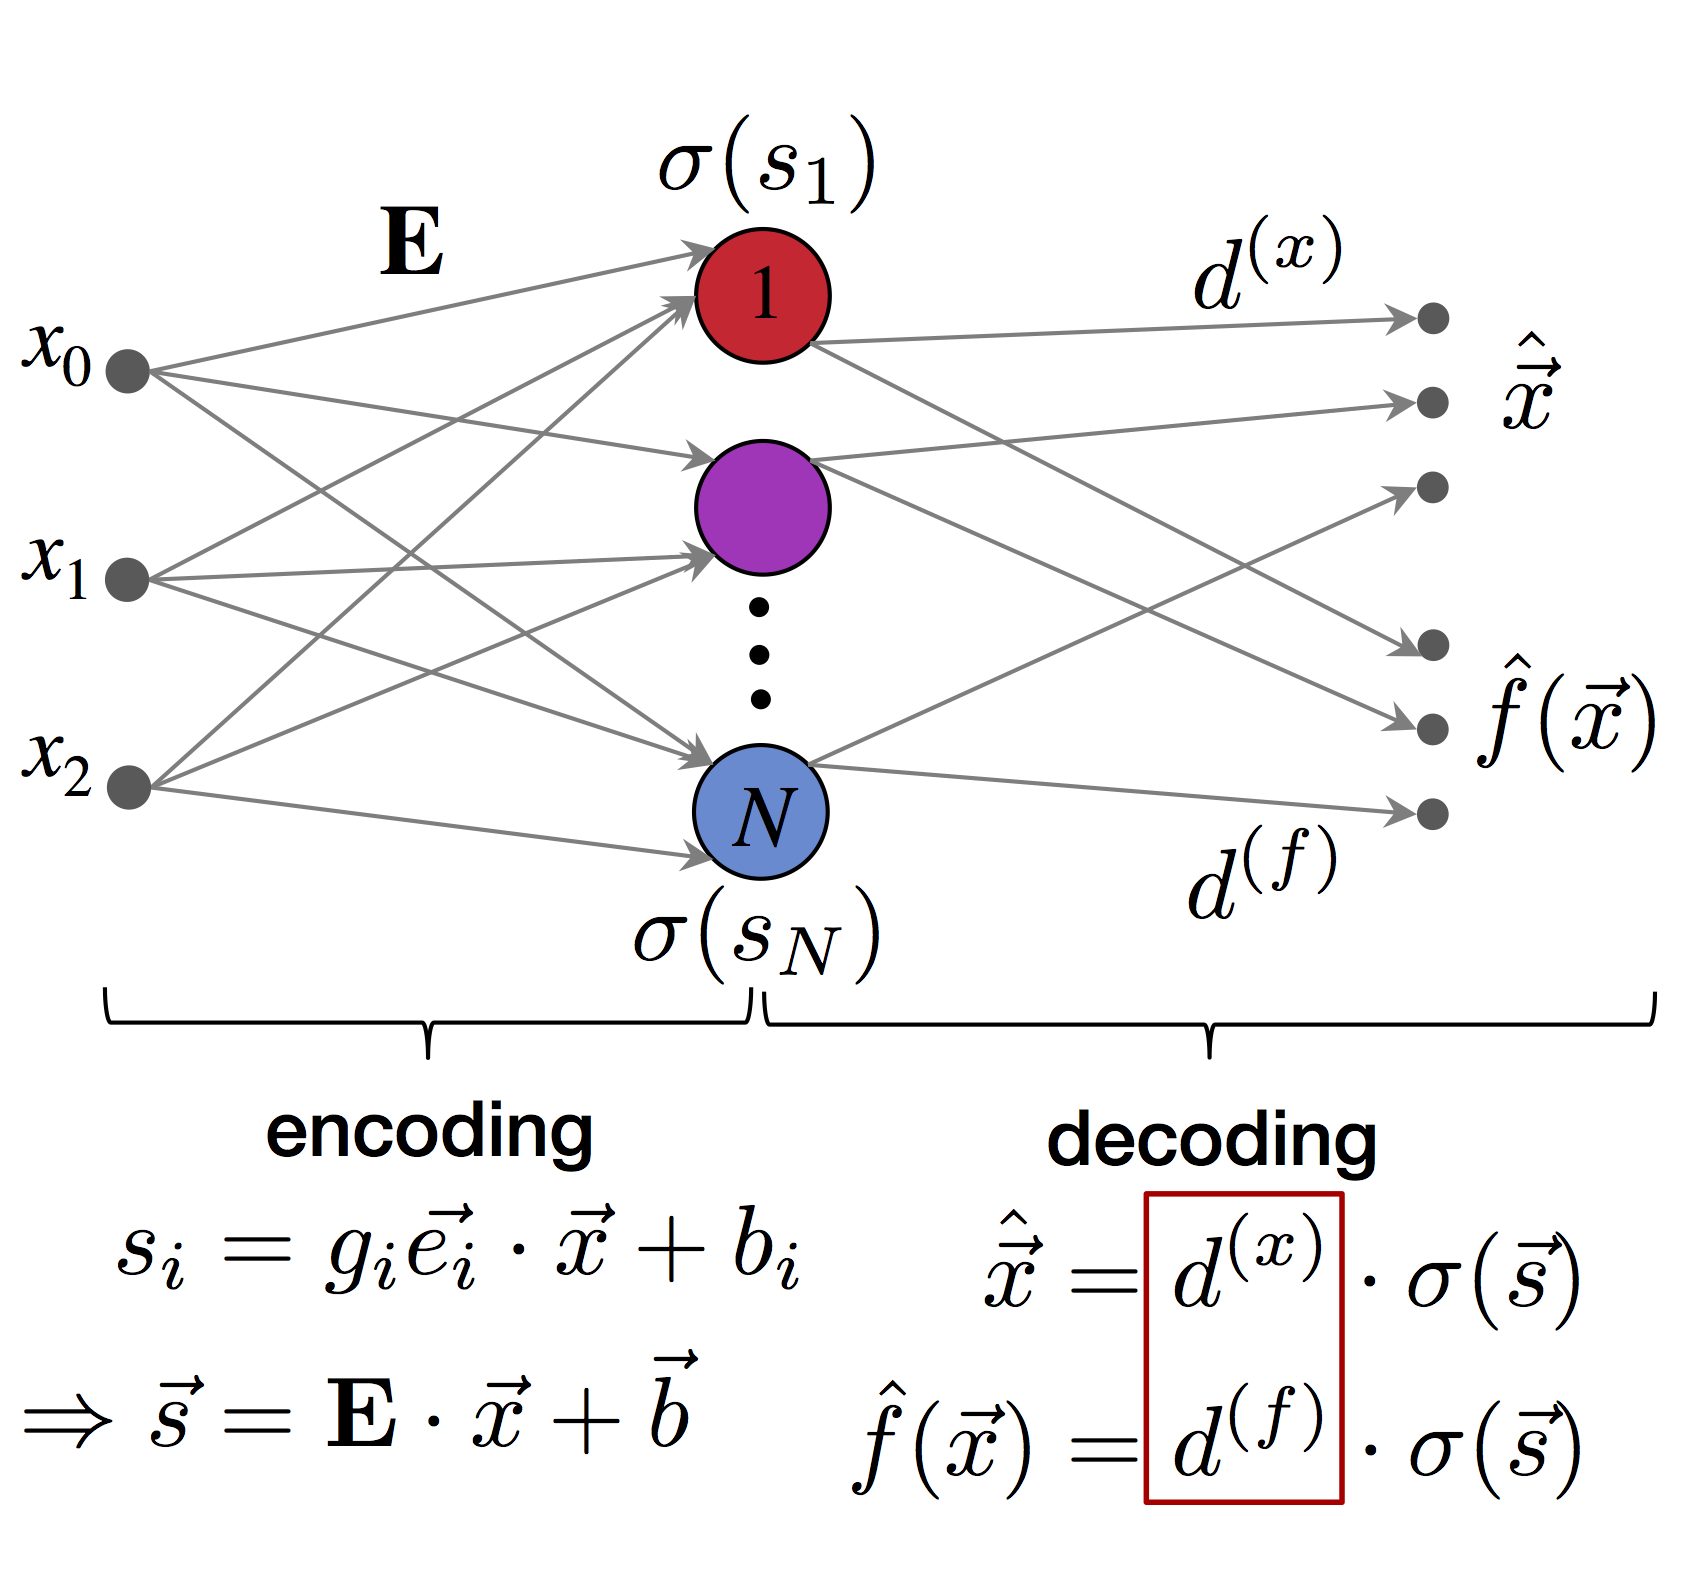
\includegraphics{Fig1.png}
\caption{}
\end{figure}

As mentioned, nengo decodes a function \(h(\vec x)\) from the population
of neurons by a linear decoding strategy, i.e.~a matrix \(d^{(h)}\)
resulting in an estimator \(\hat h(\vec x)\):

\[\hat h(\vec x) = d^{(h)} \vec y\] where
\(y_i = \sigma(s_i) = \sigma(g_i \vec e_i \cdot \vec x + b_i)\\\).

This matrix \(d^{(h)}\) is uniquely dependent on the encoder strategy,
the neuron's transfer function \(\sigma\) and the function \(h\). As a
result, it can be pre-computed before any real-time simulation. Namely,
it attempts to minimize the following objective function:

\[J = \int \left\lVert d^{(h)}\vec y - h(\vec x)\right\rVert \mathrm{d}\vec x\]
where the integral is over the desired range of values of \(\vec x\).

The minimum can be calculated via the Moore-Penrose pseudoinverse method
(\href{https://doi.org/10.3389/neuro.11.007.2009}{Stewart et al. Front
Neuroinform. 3 (2009)}):

\[ 
\Gamma_{ij} = \int y_i y_j \mathrm{d}\vec x
\] \[
\Upsilon_i = \int y_i h(\vec x) \mathrm{d} \vec x
\] \[
d^{(h)} = \Gamma^{-1} \cdot \Upsilon
\]

\subsection{Weight matrix}\label{weight-matrix}

\begin{figure}
\centering
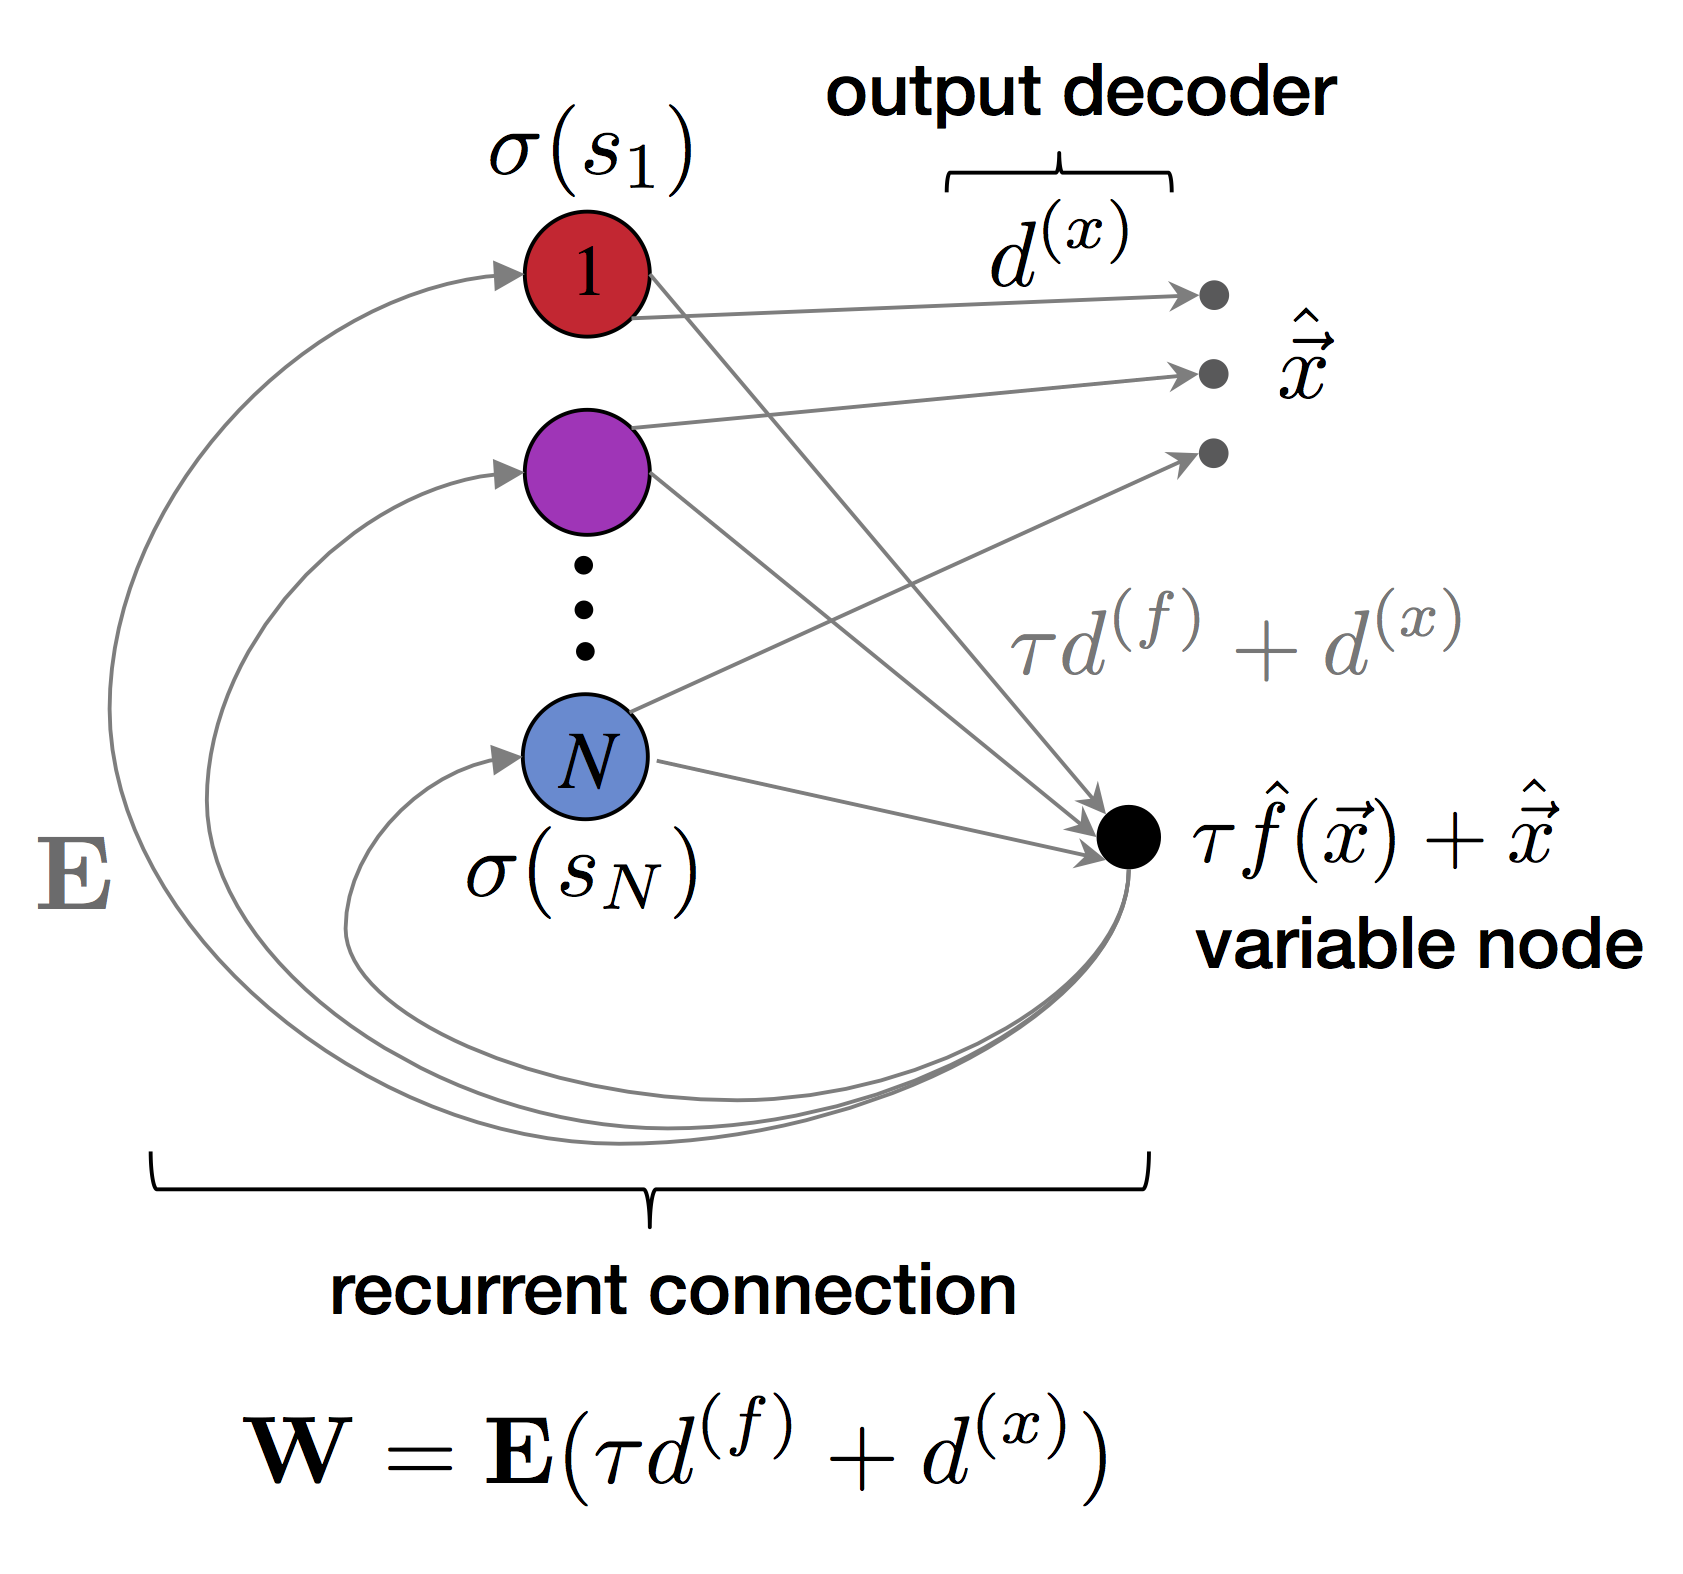
\includegraphics{Fig2.png}
\caption{}
\end{figure}

If we add an all-to-all recurrent connection to the neural population,
their collective dynamics is described by the following ODE system:

\[ \tau  \dot{\vec s} + \vec s =\overline{\overline{W}} \sigma(\vec s) + \vec I \]
where \(\overline{\overline{W}}\) is the weight matrix and \(\vec I\) a
bias vector.

Nengo sets
\(\overline{\overline{W}} = \overline{\overline{E}} (d^{(x)} + \tau d^{(f)})\)
and \(\vec I = \vec b\), where
\(\overline{\overline{E}}_{ij} = (\vec e_i)_j\). When applied to the ODE
above, it is easy to see that one can recover the Lorenz system:

\[ 
\overline{\overline{E}} (\tau  \dot{\vec x} + \vec x) = \overline{\overline{E}} (\hat{\vec x} + \tau \hat{f}(\vec x))
\]

\[ 
\Longrightarrow \dot{\vec x} = f(\vec x) + \epsilon(\vec x)
\] where
\(\epsilon(\vec x) = (1/\tau) (\hat{\vec x} - \vec x) + \hat{f}(\vec x) - f(\vec x)\).

Below, we show the computed weight matrix \(\overline{\overline{W}}\)
for this system.

    \begin{Verbatim}[commandchars=\\\{\}]
{\color{incolor}In [{\color{incolor}4}]:} \PY{c+c1}{\PYZsh{} The weight probe is sim.data[weight\PYZus{}probe][0,:,:], }
        \PY{c+c1}{\PYZsh{} but that gives the best approx to (x0, x1, x2)}
        \PY{c+c1}{\PYZsh{} What we actually want is the interconnection matrix.}
        \PY{c+c1}{\PYZsh{} For that, you need to encode this vector using the encoders variable.}
        \PY{n}{weight\PYZus{}matrix} \PY{o}{=} \PY{n}{np}\PY{o}{.}\PY{n}{dot}\PY{p}{(}\PY{n}{encoders}\PY{p}{,} \PY{n}{sim}\PY{o}{.}\PY{n}{data}\PY{p}{[}\PY{n}{weight\PYZus{}probe}\PY{p}{]}\PY{p}{[}\PY{l+m+mi}{0}\PY{p}{,}\PY{p}{:}\PY{p}{,}\PY{p}{:}\PY{p}{]}\PY{p}{)}
        
        \PY{n}{saving} \PY{o}{=} \PY{k+kc}{False}
        \PY{k}{if} \PY{n}{saving}\PY{p}{:}
            \PY{n}{pp} \PY{o}{=} \PY{n}{PdfPages}\PY{p}{(}\PY{l+s+s1}{\PYZsq{}}\PY{l+s+s1}{weight\PYZus{}matrix.pdf}\PY{l+s+s1}{\PYZsq{}}\PY{p}{)}
        \PY{n}{fig} \PY{o}{=} \PY{n}{plt}\PY{o}{.}\PY{n}{figure}\PY{p}{(}\PY{l+m+mi}{3}\PY{p}{,} \PY{n}{figsize}\PY{o}{=}\PY{p}{(}\PY{l+m+mi}{3}\PY{p}{,}\PY{l+m+mi}{3}\PY{p}{)}\PY{p}{,} \PY{n}{dpi}\PY{o}{=}\PY{l+m+mi}{72}\PY{p}{)}
        \PY{n}{plt}\PY{o}{.}\PY{n}{imshow}\PY{p}{(}\PY{n}{weight\PYZus{}matrix}\PY{p}{,} \PY{n}{cmap}\PY{o}{=}\PY{l+s+s1}{\PYZsq{}}\PY{l+s+s1}{bwr}\PY{l+s+s1}{\PYZsq{}}\PY{p}{,} \PY{n}{interpolation}\PY{o}{=}\PY{l+s+s1}{\PYZsq{}}\PY{l+s+s1}{nearest}\PY{l+s+s1}{\PYZsq{}}\PY{p}{)}
        \PY{n}{plt}\PY{o}{.}\PY{n}{colorbar}\PY{p}{(}\PY{p}{)}
        \PY{k}{if} \PY{n}{saving}\PY{p}{:}
            \PY{n}{pp}\PY{o}{.}\PY{n}{savefig}\PY{p}{(}\PY{p}{)}
            \PY{n}{pp}\PY{o}{.}\PY{n}{close}\PY{p}{(}\PY{p}{)}
        \PY{n+nb}{print}\PY{p}{(}\PY{l+s+s1}{\PYZsq{}}\PY{l+s+s1}{Max weight sum is}\PY{l+s+s1}{\PYZsq{}}\PY{p}{,} \PY{n}{np}\PY{o}{.}\PY{n}{max}\PY{p}{(}\PY{n}{np}\PY{o}{.}\PY{n}{abs}\PY{p}{(}\PY{n}{weight\PYZus{}matrix}\PY{p}{)}\PY{p}{,} \PY{n}{axis}\PY{o}{=}\PY{l+m+mi}{1}\PY{p}{)}\PY{p}{)}
\end{Verbatim}

    \begin{Verbatim}[commandchars=\\\{\}]
Max weight sum is [ 1195.11526203  1234.71946625  1209.20545697  1216.83446327  1195.11526203
  1234.71946625  1209.20545697  1216.83446327  1195.11526203  1234.71946625
  1209.20545697  1216.83446327  1195.11526203  1234.71946625  1209.20545697
  1216.83446327  1195.11526203  1234.71946625  1209.20545697  1216.83446327
  1195.11526203  1234.71946625  1209.20545697  1216.83446327]

    \end{Verbatim}

    \begin{center}
    \adjustimage{max size={0.9\linewidth}{0.9\paperheight}}{Neuromorphic_Silicon_Photonics_files/Neuromorphic_Silicon_Photonics_9_1.png}
    \end{center}
    { \hspace*{\fill} \\}
    
\section{Solved ODE: Decoded ODE
traces}\label{solved-ode-decoded-ode-traces}

Now let's plot the decoded outputs of the neuron look like when we
decode for \(\vec{x}\) using \(d^{(x)} \vec s\). Observe the emergence
of the Lorenz attractor butterfly shape.

    \begin{Verbatim}[commandchars=\\\{\}]
{\color{incolor}In [{\color{incolor}5}]:} \PY{k+kn}{from} \PY{n+nn}{mpl\PYZus{}toolkits}\PY{n+nn}{.}\PY{n+nn}{mplot3d} \PY{k}{import} \PY{n}{Axes3D}
        \PY{n}{saving} \PY{o}{=} \PY{k+kc}{False}
        
        \PY{k}{if} \PY{n}{saving}\PY{p}{:}
            \PY{n}{pp} \PY{o}{=} \PY{n}{PdfPages}\PY{p}{(}\PY{l+s+s1}{\PYZsq{}}\PY{l+s+s1}{lorenz\PYZus{}system\PYZus{}3d.pdf}\PY{l+s+s1}{\PYZsq{}}\PY{p}{)}
        \PY{n}{fig} \PY{o}{=} \PY{n}{plt}\PY{o}{.}\PY{n}{figure}\PY{p}{(}\PY{l+m+mi}{0}\PY{p}{,} \PY{n}{figsize}\PY{o}{=}\PY{p}{(}\PY{l+m+mi}{6}\PY{p}{,}\PY{l+m+mf}{4.8}\PY{p}{)}\PY{p}{,} \PY{n}{dpi}\PY{o}{=}\PY{l+m+mi}{72}\PY{p}{)}
        \PY{n}{ax} \PY{o}{=} \PY{n}{fig}\PY{o}{.}\PY{n}{add\PYZus{}subplot}\PY{p}{(}\PY{l+m+mi}{111}\PY{p}{,} \PY{n}{projection}\PY{o}{=}\PY{l+s+s1}{\PYZsq{}}\PY{l+s+s1}{3d}\PY{l+s+s1}{\PYZsq{}}\PY{p}{)}
        \PY{n}{dat3d} \PY{o}{=} \PY{p}{(}\PY{n}{sim}\PY{o}{.}\PY{n}{data}\PY{p}{[}\PY{n}{variable\PYZus{}probe}\PY{p}{]}\PY{p}{[}\PY{p}{:}\PY{p}{,} \PY{n}{dim}\PY{p}{]} \PY{k}{for} \PY{n}{dim} \PY{o+ow}{in} \PY{n+nb}{range}\PY{p}{(}\PY{l+m+mi}{3}\PY{p}{)}\PY{p}{)}
        \PY{n}{ax}\PY{o}{.}\PY{n}{plot}\PY{p}{(}\PY{o}{*}\PY{n}{dat3d}\PY{p}{,} \PY{n}{linewidth} \PY{o}{=} \PY{l+m+mf}{0.5}\PY{p}{)}
        \PY{n}{ax}\PY{o}{.}\PY{n}{set\PYZus{}xlabel}\PY{p}{(}\PY{l+s+s1}{\PYZsq{}}\PY{l+s+s1}{\PYZdl{}x\PYZus{}0\PYZdl{} (a.u.)}\PY{l+s+s1}{\PYZsq{}}\PY{p}{,} \PY{n}{fontsize}\PY{o}{=}\PY{l+m+mi}{12}\PY{p}{)}
        \PY{n}{ax}\PY{o}{.}\PY{n}{set\PYZus{}ylabel}\PY{p}{(}\PY{l+s+s1}{\PYZsq{}}\PY{l+s+s1}{\PYZdl{}x\PYZus{}1\PYZdl{} (a.u.)}\PY{l+s+s1}{\PYZsq{}}\PY{p}{,} \PY{n}{fontsize}\PY{o}{=}\PY{l+m+mi}{12}\PY{p}{)}
        \PY{n}{ax}\PY{o}{.}\PY{n}{set\PYZus{}zlabel}\PY{p}{(}\PY{l+s+s1}{\PYZsq{}}\PY{l+s+s1}{\PYZdl{}x\PYZus{}2\PYZdl{} (a.u.)}\PY{l+s+s1}{\PYZsq{}}\PY{p}{,} \PY{n}{fontsize}\PY{o}{=}\PY{l+m+mi}{12}\PY{p}{)}
        \PY{k}{for} \PY{n}{xlabel\PYZus{}i} \PY{o+ow}{in} \PY{n}{ax}\PY{o}{.}\PY{n}{get\PYZus{}xticklabels}\PY{p}{(}\PY{p}{)}\PY{p}{:}
            \PY{n}{xlabel\PYZus{}i}\PY{o}{.}\PY{n}{set\PYZus{}fontsize}\PY{p}{(}\PY{l+m+mf}{12.0}\PY{p}{)}
        \PY{k}{for} \PY{n}{ylabel\PYZus{}i} \PY{o+ow}{in} \PY{n}{ax}\PY{o}{.}\PY{n}{get\PYZus{}yticklabels}\PY{p}{(}\PY{p}{)}\PY{p}{:}
            \PY{n}{ylabel\PYZus{}i}\PY{o}{.}\PY{n}{set\PYZus{}fontsize}\PY{p}{(}\PY{l+m+mf}{12.0}\PY{p}{)}
        \PY{k}{for} \PY{n}{zlabel\PYZus{}i} \PY{o+ow}{in} \PY{n}{ax}\PY{o}{.}\PY{n}{get\PYZus{}zticklabels}\PY{p}{(}\PY{p}{)}\PY{p}{:}
            \PY{n}{zlabel\PYZus{}i}\PY{o}{.}\PY{n}{set\PYZus{}fontsize}\PY{p}{(}\PY{l+m+mf}{12.0}\PY{p}{)}
        
        \PY{n}{plt}\PY{o}{.}\PY{n}{tight\PYZus{}layout}\PY{p}{(}\PY{p}{)}
        \PY{k}{if} \PY{n}{saving}\PY{p}{:}
            \PY{n}{pp}\PY{o}{.}\PY{n}{savefig}\PY{p}{(}\PY{p}{)}
            \PY{n}{pp}\PY{o}{.}\PY{n}{close}\PY{p}{(}\PY{p}{)}
            \PY{n}{pp} \PY{o}{=} \PY{n}{PdfPages}\PY{p}{(}\PY{l+s+s1}{\PYZsq{}}\PY{l+s+s1}{lorenz\PYZus{}time\PYZus{}traces.pdf}\PY{l+s+s1}{\PYZsq{}}\PY{p}{)}
        \PY{n}{fig} \PY{o}{=} \PY{n}{plt}\PY{o}{.}\PY{n}{figure}\PY{p}{(}\PY{l+m+mi}{1}\PY{p}{,} \PY{n}{figsize}\PY{o}{=}\PY{p}{(}\PY{l+m+mi}{6}\PY{p}{,}\PY{l+m+mf}{4.8}\PY{p}{)}\PY{p}{,} \PY{n}{dpi}\PY{o}{=}\PY{l+m+mi}{72}\PY{p}{)}
        \PY{k}{for} \PY{n}{variable}\PY{p}{,} \PY{n}{label} \PY{o+ow}{in} \PY{n+nb}{zip}\PY{p}{(}\PY{n}{sim}\PY{o}{.}\PY{n}{data}\PY{p}{[}\PY{n}{variable\PYZus{}probe}\PY{p}{]}\PY{o}{.}\PY{n}{T}\PY{p}{,} 
                                   \PY{p}{[}\PY{l+s+s1}{\PYZsq{}}\PY{l+s+s1}{\PYZdl{}x\PYZus{}0\PYZdl{}}\PY{l+s+s1}{\PYZsq{}}\PY{p}{,} \PY{l+s+s1}{\PYZsq{}}\PY{l+s+s1}{\PYZdl{}x\PYZus{}1\PYZdl{}}\PY{l+s+s1}{\PYZsq{}}\PY{p}{,} \PY{l+s+s1}{\PYZsq{}}\PY{l+s+s1}{\PYZdl{}x\PYZus{}2\PYZdl{}}\PY{l+s+s1}{\PYZsq{}}\PY{p}{]}\PY{p}{)}\PY{p}{:}
            \PY{n}{plt}\PY{o}{.}\PY{n}{plot}\PY{p}{(}\PY{n}{sim}\PY{o}{.}\PY{n}{trange}\PY{p}{(}\PY{p}{)}\PY{p}{,} \PY{n}{variable}\PY{p}{,} \PY{n}{label}\PY{o}{=}\PY{n}{label}\PY{p}{,} \PY{n}{linewidth} \PY{o}{=} \PY{l+m+mf}{0.8}\PY{p}{)}
        \PY{c+c1}{\PYZsh{} for dvar in sim.data[delay\PYZus{}probe].T:}
        \PY{c+c1}{\PYZsh{}     plt.plot(sim.trange(), dvar)}
        \PY{n}{ax} \PY{o}{=} \PY{n}{plt}\PY{o}{.}\PY{n}{gca}\PY{p}{(}\PY{p}{)}
        \PY{n}{plt}\PY{o}{.}\PY{n}{legend}\PY{p}{(}\PY{n}{bbox\PYZus{}to\PYZus{}anchor}\PY{o}{=}\PY{p}{(}\PY{l+m+mf}{0.}\PY{p}{,} \PY{o}{.}\PY{l+m+mi}{02}\PY{p}{,} \PY{l+m+mf}{1.}\PY{p}{,} \PY{o}{.}\PY{l+m+mi}{102}\PY{p}{)}\PY{p}{,} \PY{n}{loc}\PY{o}{=}\PY{l+s+s1}{\PYZsq{}}\PY{l+s+s1}{lower center}\PY{l+s+s1}{\PYZsq{}}\PY{p}{,}
                   \PY{n}{ncol}\PY{o}{=}\PY{l+m+mi}{3}\PY{p}{,} \PY{n}{borderaxespad}\PY{o}{=}\PY{l+m+mf}{0.}\PY{p}{,} \PY{n}{fontsize}\PY{o}{=}\PY{l+m+mi}{12}\PY{p}{)}
        \PY{n}{plt}\PY{o}{.}\PY{n}{xlabel}\PY{p}{(}\PY{l+s+s1}{\PYZsq{}}\PY{l+s+s1}{Time (ns)}\PY{l+s+s1}{\PYZsq{}}\PY{p}{,} \PY{n}{fontsize}\PY{o}{=}\PY{l+m+mi}{12}\PY{p}{)}
        \PY{n}{plt}\PY{o}{.}\PY{n}{ylabel}\PY{p}{(}\PY{l+s+s1}{\PYZsq{}}\PY{l+s+s1}{Simulation variables, \PYZdl{}x\PYZdl{} (a.u.)}\PY{l+s+s1}{\PYZsq{}}\PY{p}{,} \PY{n}{fontsize}\PY{o}{=}\PY{l+m+mi}{12}\PY{p}{)}
        \PY{k}{for} \PY{n}{xlabel\PYZus{}i} \PY{o+ow}{in} \PY{n}{ax}\PY{o}{.}\PY{n}{get\PYZus{}xticklabels}\PY{p}{(}\PY{p}{)}\PY{p}{:}
            \PY{n}{xlabel\PYZus{}i}\PY{o}{.}\PY{n}{set\PYZus{}fontsize}\PY{p}{(}\PY{l+m+mf}{12.0}\PY{p}{)}
        \PY{k}{for} \PY{n}{ylabel\PYZus{}i} \PY{o+ow}{in} \PY{n}{ax}\PY{o}{.}\PY{n}{get\PYZus{}yticklabels}\PY{p}{(}\PY{p}{)}\PY{p}{:}
            \PY{n}{ylabel\PYZus{}i}\PY{o}{.}\PY{n}{set\PYZus{}fontsize}\PY{p}{(}\PY{l+m+mf}{12.0}\PY{p}{)}
        \PY{n}{plt}\PY{o}{.}\PY{n}{tight\PYZus{}layout}\PY{p}{(}\PY{p}{)}
        \PY{n}{plt}\PY{o}{.}\PY{n}{xlim}\PY{p}{(}\PY{p}{(}\PY{l+m+mi}{0}\PY{p}{,}\PY{n+nb}{max}\PY{p}{(}\PY{n}{sim}\PY{o}{.}\PY{n}{trange}\PY{p}{(}\PY{p}{)}\PY{p}{)}\PY{p}{)}\PY{p}{)}
        \PY{c+c1}{\PYZsh{} plt.ylim(15*np.array([\PYZhy{}1,1]))}
        \PY{k}{if} \PY{n}{saving}\PY{p}{:}
            \PY{n}{pp}\PY{o}{.}\PY{n}{savefig}\PY{p}{(}\PY{p}{)}
            \PY{n}{pp}\PY{o}{.}\PY{n}{close}\PY{p}{(}\PY{p}{)}
\end{Verbatim}

    \begin{center}
    \adjustimage{max size={0.9\linewidth}{0.9\paperheight}}{Neuromorphic_Silicon_Photonics_files/Neuromorphic_Silicon_Photonics_11_0.png}
    \end{center}
    { \hspace*{\fill} \\}
    
    \begin{center}
    \adjustimage{max size={0.9\linewidth}{0.9\paperheight}}{Neuromorphic_Silicon_Photonics_files/Neuromorphic_Silicon_Photonics_11_1.png}
    \end{center}
    { \hspace*{\fill} \\}
    
\subsection{Neural state time traces}\label{neural-state-time-traces}

Let's plot the undecoded state of each neuron i: \(\vec s_i\). Observe
which neurons are active vs which aren't.

    \begin{Verbatim}[commandchars=\\\{\}]
{\color{incolor}In [{\color{incolor}7}]:} \PY{n}{saving} \PY{o}{=} \PY{k+kc}{False}
        \PY{k}{if} \PY{n}{saving}\PY{p}{:}
            \PY{n}{pp} \PY{o}{=} \PY{n}{PdfPages}\PY{p}{(}\PY{l+s+s1}{\PYZsq{}}\PY{l+s+s1}{MZM\PYZus{}time\PYZus{}traces.pdf}\PY{l+s+s1}{\PYZsq{}}\PY{p}{)}
        \PY{n}{fig} \PY{o}{=} \PY{n}{plt}\PY{o}{.}\PY{n}{figure}\PY{p}{(}\PY{l+m+mi}{2}\PY{p}{,} \PY{n}{figsize}\PY{o}{=}\PY{p}{(}\PY{l+m+mi}{6}\PY{p}{,}\PY{l+m+mi}{6}\PY{p}{)}\PY{p}{,} \PY{n}{dpi}\PY{o}{=}\PY{l+m+mi}{72}\PY{p}{)}
        \PY{n}{ax} \PY{o}{=} \PY{n}{plt}\PY{o}{.}\PY{n}{gca}\PY{p}{(}\PY{p}{)}
        
        \PY{n}{cm} \PY{o}{=} \PY{n}{plt}\PY{o}{.}\PY{n}{get\PYZus{}cmap}\PY{p}{(}\PY{l+s+s1}{\PYZsq{}}\PY{l+s+s1}{Paired}\PY{l+s+s1}{\PYZsq{}}\PY{p}{)} 
        \PY{n}{cNorm}  \PY{o}{=} \PY{n}{colors}\PY{o}{.}\PY{n}{Normalize}\PY{p}{(}\PY{n}{vmin}\PY{o}{=}\PY{l+m+mi}{0}\PY{p}{,} \PY{n}{vmax}\PY{o}{=}\PY{n}{num\PYZus{}neurons}\PY{p}{)}
        \PY{n}{scalarMap} \PY{o}{=} \PY{n}{cmx}\PY{o}{.}\PY{n}{ScalarMappable}\PY{p}{(}\PY{n}{norm}\PY{o}{=}\PY{n}{cNorm}\PY{p}{,} \PY{n}{cmap}\PY{o}{=}\PY{n}{cm}\PY{p}{)}
        \PY{k}{for} \PY{n}{i} \PY{o+ow}{in} \PY{n+nb}{range}\PY{p}{(}\PY{n}{num\PYZus{}neurons}\PY{p}{)}\PY{p}{:}
            \PY{n}{colorVal} \PY{o}{=} \PY{n}{scalarMap}\PY{o}{.}\PY{n}{to\PYZus{}rgba}\PY{p}{(}\PY{n}{i}\PY{p}{)}
            \PY{n}{plt}\PY{o}{.}\PY{n}{plot}\PY{p}{(}\PY{n}{sim}\PY{o}{.}\PY{n}{trange}\PY{p}{(}\PY{p}{)}\PY{p}{,} \PY{n}{sim}\PY{o}{.}\PY{n}{data}\PY{p}{[}\PY{n}{state\PYZus{}probe}\PY{p}{]}\PY{p}{[}\PY{p}{:}\PY{p}{,} \PY{n}{i}\PY{p}{]}\PY{o}{/}\PY{n}{max\PYZus{}transmission} \PY{o}{+} \PY{p}{(}\PY{n}{i}\PY{o}{+}\PY{o}{.}\PY{l+m+mi}{5}\PY{p}{)}\PY{p}{,} 
                     \PY{n}{lw}\PY{o}{=}\PY{o}{.}\PY{l+m+mi}{5}\PY{p}{,} \PY{n}{color}\PY{o}{=}\PY{l+s+s1}{\PYZsq{}}\PY{l+s+s1}{k}\PY{l+s+s1}{\PYZsq{}}\PY{p}{)}
        \PY{c+c1}{\PYZsh{} plt.xlabel(\PYZsq{}Real time (ns)\PYZsq{})}
        \PY{n}{plt}\PY{o}{.}\PY{n}{ylabel}\PY{p}{(}\PY{l+s+s1}{\PYZsq{}}\PY{l+s+s1}{Modulator neuron index}\PY{l+s+s1}{\PYZsq{}}\PY{p}{,} \PY{n}{fontsize}\PY{o}{=}\PY{l+m+mi}{12}\PY{p}{)}
        \PY{n}{plt}\PY{o}{.}\PY{n}{xticks}\PY{p}{(}\PY{p}{[}\PY{p}{]}\PY{p}{)}
        \PY{n}{plt}\PY{o}{.}\PY{n}{yticks}\PY{p}{(}\PY{l+m+mi}{1} \PY{o}{+} \PY{n}{np}\PY{o}{.}\PY{n}{arange}\PY{p}{(}\PY{n}{num\PYZus{}neurons}\PY{p}{)}\PY{p}{)}
        \PY{n}{ax}\PY{o}{.}\PY{n}{set\PYZus{}yticklabels}\PY{p}{(}\PY{n}{ax}\PY{o}{.}\PY{n}{get\PYZus{}yticks}\PY{p}{(}\PY{p}{)}\PY{p}{,} \PY{n}{fontsize}\PY{o}{=}\PY{l+m+mi}{8}\PY{p}{)}
        \PY{k}{for} \PY{n}{s} \PY{o+ow}{in} \PY{n}{ax}\PY{o}{.}\PY{n}{spines}\PY{p}{:}
            \PY{n}{ax}\PY{o}{.}\PY{n}{spines}\PY{p}{[}\PY{n}{s}\PY{p}{]}\PY{o}{.}\PY{n}{set\PYZus{}visible}\PY{p}{(}\PY{k+kc}{False}\PY{p}{)}
        
        \PY{k}{if} \PY{n}{saving}\PY{p}{:}
            \PY{n}{pp}\PY{o}{.}\PY{n}{savefig}\PY{p}{(}\PY{p}{)}
            \PY{n}{pp}\PY{o}{.}\PY{n}{close}\PY{p}{(}\PY{p}{)}
\end{Verbatim}

    \begin{center}
    \adjustimage{max size={0.9\linewidth}{0.9\paperheight}}{Neuromorphic_Silicon_Photonics_files/Neuromorphic_Silicon_Photonics_13_0.png}
    \end{center}
    { \hspace*{\fill} \\}
    
    \begin{Verbatim}[commandchars=\\\{\}]
{\color{incolor}In [{\color{incolor}8}]:} \PY{c+c1}{\PYZsh{} Export data for further processing in matlab.}
        \PY{k+kn}{import} \PY{n+nn}{scipy}\PY{n+nn}{.}\PY{n+nn}{io} \PY{k}{as} \PY{n+nn}{sio}
        \PY{k+kn}{import} \PY{n+nn}{os} 
        \PY{n}{dir\PYZus{}path} \PY{o}{=} \PY{n}{os}\PY{o}{.}\PY{n}{path}\PY{o}{.}\PY{n}{dirname}\PY{p}{(}\PY{n}{os}\PY{o}{.}\PY{n}{getcwd}\PY{p}{(}\PY{p}{)}\PY{p}{)}
        
        \PY{n}{dataDir} \PY{o}{=} \PY{l+s+s1}{\PYZsq{}}\PY{l+s+s1}{lightwave\PYZus{}stuff/discreteTimeLorenzFiles/ctrnn data/}\PY{l+s+s1}{\PYZsq{}}
        \PY{n}{fname} \PY{o}{=} \PY{n}{os}\PY{o}{.}\PY{n}{path}\PY{o}{.}\PY{n}{join}\PY{p}{(}\PY{n}{dir\PYZus{}path}\PY{p}{,} \PY{n}{dataDir}\PY{p}{,} \PY{l+s+s1}{\PYZsq{}}\PY{l+s+s1}{lorenz\PYZus{}signals.mat}\PY{l+s+s1}{\PYZsq{}}\PY{p}{)}
        \PY{n}{sio}\PY{o}{.}\PY{n}{savemat}\PY{p}{(}\PY{n}{fname}\PY{p}{,} \PY{p}{\PYZob{}}\PY{l+s+s1}{\PYZsq{}}\PY{l+s+s1}{time}\PY{l+s+s1}{\PYZsq{}}\PY{p}{:}\PY{n}{sim}\PY{o}{.}\PY{n}{trange}\PY{p}{(}\PY{p}{)}\PY{p}{,} \PY{l+s+s1}{\PYZsq{}}\PY{l+s+s1}{x}\PY{l+s+s1}{\PYZsq{}}\PY{p}{:}\PY{n}{sim}\PY{o}{.}\PY{n}{data}\PY{p}{[}\PY{n}{variable\PYZus{}probe}\PY{p}{]}\PY{o}{.}\PY{n}{T}\PY{p}{\PYZcb{}}\PY{p}{)}
        \PY{n}{sio}\PY{o}{.}\PY{n}{whosmat}\PY{p}{(}\PY{n}{fname}\PY{p}{)}
\end{Verbatim}

            \begin{Verbatim}[commandchars=\\\{\}]
{\color{outcolor}Out[{\color{outcolor}8}]:} [('time', (1, 52000), 'double'), ('x', (3, 52000), 'double')]
\end{Verbatim}
        
    \begin{Verbatim}[commandchars=\\\{\}]
{\color{incolor}In [{\color{incolor} }]:} 
\end{Verbatim}


    % Add a bibliography block to the postdoc
    
    
    
    \end{document}
